\documentclass{book}
\usepackage{physics}
\usepackage{graphicx}
\usepackage{caption}
\usepackage{amsmath}
\usepackage{bm}
\usepackage{framed}
\usepackage{authblk}
\usepackage{empheq}
\usepackage{amsfonts}
\usepackage{esint}
\usepackage[makeroom]{cancel}
\usepackage{dsfont}
\usepackage{centernot}
\usepackage{mathtools}
\usepackage{bigints}
\usepackage{amsthm}
\theoremstyle{definition}
\newtheorem{defn}{Definition}[section]
\newtheorem{prop}{Proposition}[section]
\newtheorem{rmk}{Remark}[section]
\newtheorem{thm}{Theorem}[section]
\newtheorem{exmp}{Example}[section]
\newtheorem{prob}{Problem}[section]
\newtheorem{sln}{Solution}[section]
\newtheorem*{prob*}{Problem}
\newtheorem{exer}{Exercise}[section]
\newtheorem*{exer*}{Exercise}
\newtheorem*{sln*}{Solution}
\usepackage{empheq}
\usepackage{hyperref}
\usepackage{tensor}
\usepackage{xcolor}
\hypersetup{
	colorlinks,
	linkcolor={black!50!black},
	citecolor={blue!50!black},
	urlcolor={blue!80!black}
}


\newcommand*\widefbox[1]{\fbox{\hspace{2em}#1\hspace{2em}}}

\newcommand{\p}{\partial}
\newcommand{\R}{\mathbb{R}}
\newcommand{\C}{\mathbb{C}}
\newcommand{\lag}{\mathcal{L}}
\newcommand{\nn}{\nonumber}
\newcommand{\had}{\mathcal{H}}
\newcommand{\M}{\mathcal{M}}
\newcommand{\I}{\mathcal{I}}
\newcommand{\K}{\mathcal{K}}
\newcommand{\F}{\mathcal{F}}
\newcommand{\w}{\omega}
\newcommand{\lam}{\lambda}
\newcommand{\al}{\alpha}
\newcommand{\be}{\beta}
\newcommand{\x}{\xi}

\newcommand{\G}{\mathcal{G}}

\newcommand{\f}[2]{\frac{#1}{#2}}

\newcommand{\ift}{\infty}

\newcommand{\lp}{\left(}
\newcommand{\rp}{\right)}

\newcommand{\lb}{\left[}
\newcommand{\rb}{\right]}

\newcommand{\lc}{\left\{}
\newcommand{\rc}{\right\}}


\newcommand{\V}{\mathbf{V}}
\newcommand{\U}{\mathcal{U}}
\newcommand{\Id}{\mathcal{I}}
\newcommand{\D}{\mathcal{D}}
\newcommand{\Z}{\mathcal{Z}}

%\setcounter{chapter}{-1}


\makeatletter
\renewcommand{\@chapapp}{Part}
%\renewcommand\thechapter{$\bf{\ket{\arabic{chapter}}}$}
%\renewcommand\thesection{$\bf{\ket{\arabic{section}}}$}
%\renewcommand\thesubsection{$\bf{\ket{\arabic{subsection}}}$}
%\renewcommand\thesubsubsection{$\bf{\ket{\arabic{subsubsection}}}$}
\makeatother



\usepackage{subfig}
\usepackage{listings}
\captionsetup[lstlisting]{margin=0cm,format=hang,font=small,format=plain,labelfont={bf,up},textfont={it}}
\renewcommand*{\lstlistingname}{Code \textcolor{violet}{\textsl{Mathematica}}}
\definecolor{gris245}{RGB}{245,245,245}
\definecolor{olive}{RGB}{50,140,50}
\definecolor{brun}{RGB}{175,100,80}
\lstset{
	tabsize=4,
	frame=single,
	language=mathematica,
	basicstyle=\scriptsize\ttfamily,
	keywordstyle=\color{black},
	backgroundcolor=\color{gris245},
	commentstyle=\color{gray},
	showstringspaces=false,
	emph={
		r1,
		r2,
		epsilon,epsilon_,
		Newton,Newton_
	},emphstyle={\color{olive}},
	emph={[2]
		L,
		CouleurCourbe,
		PotentielEffectif,
		IdCourbe,
		Courbe
	},emphstyle={[2]\color{blue}},
	emph={[3]r,r_,n,n_},emphstyle={[3]\color{magenta}}
}


\begin{document}
\begin{titlepage}\centering
 \clearpage
 \title{{\textsc{\textbf{Physics at the Perimeter Institute:\\  Topics in Theoretical Physics \\ 
 				\&\\ Quantum Simulation Research}}}\\ \smallskip - A Quick Guide - \\}
 \author{\bigskip Huan Q. Bui}
  \affil{Colby College\\$\,$\\ PHYSICS \& MATHEMATICS\\ Statistics \\$\,$\\Class of 2021\\}
 \date{\today}
 \maketitle
 \thispagestyle{empty}
\end{titlepage}

\subsection*{Preface}
\addcontentsline{toc}{subsection}{Preface}

Greetings,\\

This guide is my notes from Perimeter Institute of Theoretical Physics Summer School, 2020. Topics include quantum information, thermodynamics, numerical methods, condensed matter physics, path integrals, and symmetries.\\

The text also includes reading notes for my research project at Perimeter on quantum simulation. \\

Enjoy!  



\newpage
\tableofcontents
\newpage





\chapter{Quantum Information \& Thermodynamics} 

\textbf{Instructor:} Alioscia Hamma\\

The aim of this course is to understand the thermodynamics of quantum systems and in the process to learn some fundamental tools in Quantum Information. We will focus on the topics of foundations of quantum statistical mechanics, resource theories, entanglement, fluctuation theorems, and quantum machines. 

\newpage

\section{Foundations of Quantum Statistical Mechanics - Entanglement}
\newpage

\section{Resource Theories and Quantum Information}


\newpage
\section{Quantum Thermal Operations}


\newpage
\section{Fluctuation Theorems and Quantum Information}


\newpage
\section{Quantum Thermal Machines}






\newpage
\chapter{Numerical Methods \& Condensed Matter Physics}

\textbf{Instructor:} Aaron Szasz\\

This course has two main goals: (1) to introduce some key models from condensed matter physics; and (2) to introduce some numerical approaches to studying these (and other) models.  As a precursor to these objectives, we will carefully understand many-body states and operators from the perspective of condensed matter theory.  (However, I will cover only spin models.  We will not discuss or use second quantization.)\\



Once this background is established, we will study the method of exact diagonalization and write simple python programs to find ground states, correlation functions, energy gaps, and other properties of the transverse-field Ising model and XXZ model.  We will also discuss the computational limitations of exact diagonalization.  Finally, I will introduce the concept of matrix product states, and we will see how these can be used with algorithms such as the density matrix renormalization group (DMRG) to study ground state properties for much larger systems than can be studied with exact diagonalization.




\newpage


\section{L1: Introduction to many-particle states and operators}
\newpage
\subsection{L1: Introduction to Ising and XXZ models}
\newpage
\subsection{L1: Programming basics}
\newpage
\subsection{L1 : Finding expectation values}
\newpage

\section{L2: Exact diagonalization part 1}
\newpage
\section{L2: Representing models}
\newpage
\section{L2: Finding eigenstates}
\newpage
\section{L2: Energy gaps}
\newpage
\section{L2: Phase transitions}
\newpage




\section{L3: Exact diagonalization part 2}
\newpage

\section{L3: Limitations of the method}
\newpage
\section{L3: Using symmetries}
\newpage
\section{L3: Dynamics}
\newpage




\section{L4: Matrix product states part 1}
\newpage



\section{L4: Entanglement and the singular value decomposition}
\newpage


\section{L4: What is a matrix product state and why is it useful}
\newpage





\section{L5: Matrix product states part 2}


\newpage

\section{L5: Algorithms for finding ground states using matrix product states: iTEBD }

\newpage


\section{L5: Algorithms for finding ground states using matrix product states: DMRG}

\newpage











\chapter{Path Integrals}

\textbf{Instructor:} Dan Wohns\\

The goal of this course is to introduce the path integral formulation of quantum mechanics and a few of its applications. We will begin by motivating the path integral formulation and explaining its connections to other formulations of quantum mechanics and its relation to classical mechanics. We will then explore some applications of path integrals.


\newpage

\section{Introduction to path integrals and the semi-classical limit}

Path integrals is a different yet equivalent formulation of quantum mechanics. The path integral formulation of quantum mechanics does make a connection between classical and quantum physics more clear. It also has a number of advantages, some which we will touch on later. In essence, path integrals can allow for perturbation approaches to solving problems in quantum mechanics. Path integrals also generalize quantum field theory. Solving SE is much more difficult in higher dimensions. Using a differential-equation approach to QFT is often hard. Path integrals allow for easier approaches to the same problems in QFT. \\


\subsection{Motivation \& Definition}

Consider the double slit experiment. 
\begin{figure}[!htb]
	\centering
	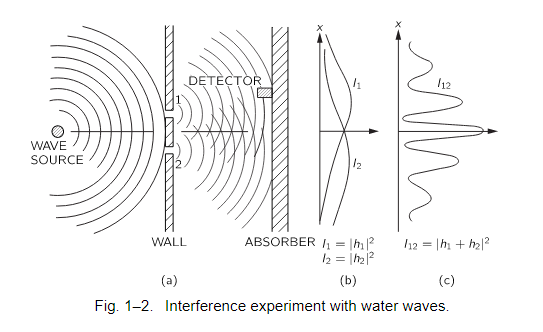
\includegraphics[scale=0.8]{double-slit}
	\caption{From Feynman's lectures of Physics}
\end{figure}

We know that the amplitude/propagator $K = A_1 + A_2$ leads to interference. \\

The basic idea behind the path integral comes from considering what happens when there are many many many more slits. This suggests that the propagator should be the sum over all paths of some functional $A[\gamma]$ that is the amplitude associated with each path:
\begin{align}
K =\sum_\gamma A[\gamma]
\end{align}
where 
\begin{align}
\boxed{K(q_f,t_f, q_i,t_i) = \bra{q_f} e^{i\had (t_f - t_f)/\hbar} \ket{q_i}}
\end{align}
is the propagator. \\


When there are infinitely many holds of infinitesimal size, the particle can be anywhere (since there's essentially no more holes), so we have the picture
\begin{figure}[!htb]
	\centering
	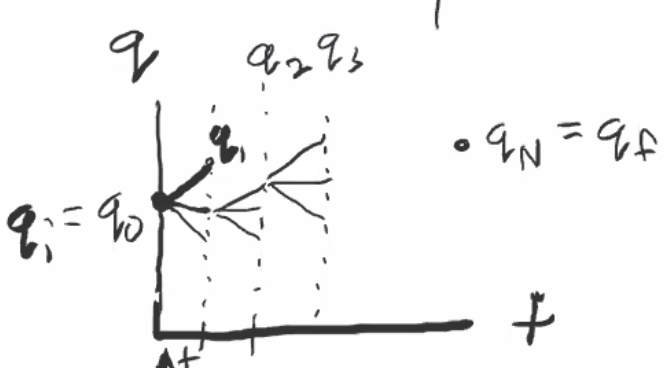
\includegraphics[scale=0.5]{time}
	\caption{From PI lecture by Dan Wohns}
\end{figure}
In this case, the sum over paths becomes an integral
\begin{align}
\sum_\gamma \to \lim_{N\to \infty}\int d q_1dq_2\dots dq_{N-1}
\end{align}


\subsection{Some properties}

\begin{prop}[Composition]
	Consider the path $\gamma_{12}$ composed of the path $\gamma_1$ followed by the path $\gamma_2$. Then
\begin{align}
A[\gamma_{12}] = A[\gamma_1] A[\gamma_2].
\end{align}
This implies (as we will see in the exercises) that
\begin{align}
K(q_f,t_f,q_i,t_i) = \int dy\,K(q_f, t_f,y,t_{int})K(y,t_{int},q_i,t_i).
\end{align}
\end{prop}


\begin{prop}[Classical Limit]
	When $\hbar \to 0$ and the action  $S \gg \hbar$, then the classical path becomes most important. 
\end{prop}


For most of the course, we will be consider actions that look like
\begin{align}
S = \int^{t_f}_{t_i} dt\, \f{1}{2}m\dot{p}^2(t) - V(q(t)).
\end{align}
The classical path satisfies the Euler-Lagrange equation: 
\begin{align}
\f{\delta S}{\delta q(t)} = 0.
\end{align}
This turns out to be 
\begin{align}
m\ddot{q} + V'(q) =0 
\end{align}
which is just Newton's second law of motion. \\


With these, we have 
\begin{align}
\int \mathfrak{D}q(t) e^{iS[q(t)]/\hbar}.
\end{align}
The composition property suggests that we should have an exponential, so that we can convert multiplication to summation. This says that all paths contribution with equal weight. So, the classical path is as important as the quantum path in the action. However, only paths such that $\delta S = 0$ contribute more to the propagator. \\

Consider the paths $q(t)$ and $q'(t) = q(t) + \eta (t)$ where $\eta(t)$ is some small perturbation, then 
\begin{align}
S[q'(t)] = S[q(t)] + \int dt\, \eta(t) \f{\delta S[q]}{\delta q(t)} + \mathcal{O}(\eta^2).
\end{align}

What happens in the general case is that 
\begin{align}
e^{iS[q]/\hbar} + e^{iS[q']/\hbar} \approx  e^{iS[q]/\hbar}\lp 1 + \exp\lb \f{i}{\hbar} \int dt\, \eta(t) \f{\delta S[t]}{\delta q(t)} \rb \rp
\end{align}
So, when $\hbar \to 0$, we get destructive interference. But if $\delta S/\delta q = 0$, we get constructive interference. So, even though all paths are equally important, it's also true that the classical path are ``more important'' than quantum paths, because they interference constructively. 








\newpage
\section{Propagator in real and imaginary time}


\newpage

\section{Perturbation theory}


\newpage

\section{Non-perturbative physics and quantum tunneling}


\newpage


\section{Topology and path integrals}


\newpage




\section{Exercises}



\noindent \textbf{1. Composition.} 
\begin{enumerate}
	\item In lecture we argued that the propagator $K$ can be written as a sum (or an integral) over paths $\gamma$ of a functional $A[\gamma]$. 
	\begin{align}
	K = \sum_\gamma A[\gamma].
	\end{align}
	Show that the propagator obeys the composition property
	\begin{align}
	K(q_f, t_f, q_i, t_i) = \int dy\, K(q_f,t_f,y,t_{int})K(y,t_{int},q_i ,t_i)
	\end{align}
	of $A$ has the factorization property
	\begin{align}
	A[\gamma_{12}] = A[\gamma_1]A[\gamma_2].
	\end{align}
	
	
	
	\begin{proof}
		Let $A$ satisfy the factorization property. Then, 
		\begin{align}
		K = \sum_{\gamma_1,\gamma_2}A[\gamma_1]A[\gamma_2] = \int \,dy \,\sum_{\gamma_1} A[\gamma_1] \sum_{\gamma_2} A[\gamma_2]
		\end{align}
		where the path $\gamma_1$ ends at $y$ and $\gamma_2$ starts at $y$. With this, it's straightforward:
		\begin{align}
		K &= \int \,dy \bra{q_f}e^{-i\had (t_f - t_{int})/\hbar}\ket{y}\bra{y} e^{-i \had (t_{int} - t_i)/\hbar} \ket{q_i}\nn\\
		&= \bra{q_f}e^{-i\had(t_f - t_{int} + t_{int} - t_i)/\hbar}\ket{q_i}   \nn\\
		&= K(q_f,t_f,q_i,t_i).
		\end{align}
		So, we're done, because from the first line we conclude
		\begin{align}
		K(q_f, t_f, q_i, t_i) = \int dy\, K(q_f,t_f,y,t_{int})K(y,t_{int},q_i ,t_i).
		\end{align}
	\end{proof}
	
	
	
	
	\item Explain why the factorization property
	\begin{align}
	A[\gamma_{12}] = A[\gamma_1]A[\gamma_2]
	\end{align}
	holds if $A[\gamma] = e^{iS[\gamma]/\hbar}$ where $S[\gamma]$ is the classical action of the trajectory $\gamma$.
	
	\begin{proof}
		We note that $S[\gamma_{12}] = S[\gamma_1] + S[\gamma_2]$ if $\gamma_{12}$ is composed of  $\gamma_1,\gamma_2$. So this factorization property follows.
	\end{proof}
	
	
	
	\item Suppose $A[\gamma] = C_1 e^{C_2 S[\gamma]}$ for some constants $C_1,C_2$. Which values of $C_1,C_2$ give rise to a composition property? 
	
	\begin{proof}
		$C_1$ must be constantly 1, so that the composition property is satisfied. $C_2$ can be any real or complex number. 
	\end{proof}
	

\end{enumerate}




\noindent \textbf{2. Classical Limit}
\begin{enumerate}
	\item Suppose $f(x)$ is a real function. Which values of $x$ provide the most important contribution to 
	\begin{itemize}
		\item $\int e^{-f(x)}\,dx$? Why? (Optional: what conditions should be placed on $f(x)$?)
		
		
		\begin{proof}
			The most important contribution to this integral is when $f$ is small, so $x$'s where $f(x)$ is small. 
		\end{proof}
	
	
		\item $\int e^{if(x)}\,dx$? Why? (Optional: what conditions should be placed on $f(x)$?)
		
		
		\begin{proof}
			The most important contribution to this integral is when $f$ changes slowly, so most comes from $x$ where $f'(x)$ small. 
		\end{proof}
	\end{itemize}



	\item The classical equation of motion for a particle with classical action $S$ is that the first-order variation vanishes:
	\begin{align}
	\delta S = 0.
	\end{align}
	A trajectory with $\delta S = 0$ is a classical trajectory. No extra conditions on the second-order variation of the action is required. Why does $A[\gamma] = e^{iS[\gamma]/\hbar}$ give the correct classical limit? 
	
	\begin{proof}
		Recall that $\delta S = 0$. So this sort of shows why $A[\gamma] = e^{iS[\gamma]/\hbar}$ works. We won't worry too much about the details here.
		
	\end{proof}
	
	\item What other choices $A[\gamma]$ give rise to the correct classical limit? Do they have a composition property? 
	
	\item Do any of the other possibilities you identified in 1(c) have the correct classical limit? 
\end{enumerate}













\newpage









































\chapter{Symmetries}

\textbf{Instructor:} Giuseppe Sellaroli\\

The aim of this course is to  explore some of the many ways in which symmetries play a role in physics. We'll start with an overview of the concept of symmetries and their description in the language of  group theory. We will then discuss continuous symmetries and infinitesimal symmetries, their fundamental role in Noether's theorem, and their formalization in terms of Lie groups and Lie algebras. In the last part of the course we will focus on symmetries in quantum theory and introduce representations of (Lie) groups and Lie algebras.


\newpage


\section{Review: Equivalence Classes}


\subsection{Equivalence relations}


An equivalence relation is a special kind of binary relation. A
(homogeneous) binary relation on a set $X$ is a way of encoding a relationship between two elements of $X$. Given a relation $R$ we use the notation $xRy$ to mean ``$x$ is related to $y$.'' \\

Examples of relations are $=,<,>, \leq, \geq$ on $\mathbb{R}$. \\

\begin{defn}[Homogeneous binary relation]
	A homogeneous binary relation on a set $X$ is a set $R \subset X \times X$ of pairs of
	elements of $X$. When $(x,y) \in R$ we say that $x$ is relate to $y$, which we also indicate with the less cumbersome notation $xRy$.  
\end{defn}

We can now define equivalence relations.



\begin{defn}[Equivalence relation]
	An equivalence relation on a set $X$ is homogeneous binary relation $R$ that satisfies the following properties:
	\begin{itemize}
		\item Reflexive: $xRx \forall x\in X$.
		\item Symmetric: $xRy \implies yRx$.
		\item Transitive: $xRy, yRz \implies xRz$
	\end{itemize}
	These properties are chosen as they encode the fundamental features of the notion of
	things being ``equivalent.''
\end{defn}

Equivalence relations are often denoted by the symbol $\sim$. In this case we read $x\sim y$ as ``$x$ is equivalent to $y$.'' 





\subsection{Equivalence Classes}

Now that we know what an equivalence relation is, we can define the extremely useful concept of equivalence class.


\begin{defn}
	Let $\sim$ be an equivalence relation on $X$. The equivalance class of $x \in X$ is the set 
	\begin{align}
	[x]_\sim = \{ y\in X \vert y\sim x   \}
	\end{align}
	of all the elements in $X$ equivalent to $x$. We often drop the subscript and just write $[x]$ if there is no risk of confusion. Note that
	\begin{align}
	[x]_\sim = [y]_\sim, \quad \forall y \in [x]_\sim,
	\end{align}
	that is we can label the equivalence class using any of its elements. The element that we
	choose as the label is called the representative of the equivalence class.
\end{defn}



Equivalence classes are essentially buckets in which we put elements of X that are equivalent
to each other. Inequivalent elements end up in different equivalence classes. One way of
thinking about this is that an equivalence class is a way to encode as a single object the
properties common to its elements, which are otherwise indistinguishable.


\begin{exmp}
	An example of equivalence relation appears in modular arithmetic. Let's consider the simplest case of the integers modulo 2. We define an equivalence relation $\sim$ on $\mathbb{Z}$ by
	\begin{align}
	x\ sim y \implies x-y = 2k, k\in \mathbb{Z},
	\end{align}
	that is $x,y$ are equivalent if they differ by a multiple of two. If you want, you can check that this is indeed an equivalence relation as an exercise. There are only two distinct equivalence classes, which are the respectively the sets of even and odd integers. The sets of integers modulo 2 is
	defined as

	\begin{align}
	\mathbb{Z}_2 = \{ [0], [1]  \}.
	\end{align}
	Although this is a set of sets, we really want to pretend that it's a set of numbers. To do
	that, we define a way to add elements in $\mathbb{Z}_2$. The obvious choice is
	\begin{align}
	[a] + [b] = [a+b],
	\end{align}
	but at this stage this expression is purely formal: since we are specifying this operation
	through the sum of the representatives of each class, we need to make sure that the definition
	is actually independent of the choice of representatives (since they should be equivalent).
	This happens all the time when dealing with equivalence classes! In this case we are fine, because of the rules of adding odd and even numbers. 
\end{exmp}



\begin{exmp}
	Here’s an example from quantum physics. Let $\had$ be the Hilbert space of a quantum theory. While extremely useful, the states $\ket{\psi} \in \had$ are not \textit{physical}, where physical is meant as something that can be measured. The physical quantities in a quantum theory are the expectation values of the observables in a given state, that is 
	\begin{align}
	\langle A \rangle_\psi = \f{\bra{\psi}A\ket{\psi}}{\braket{\psi}}.
	\end{align}
	Now consider another state $\ket{\phi} = \lambda{\psi}$, with $\lambda \in \mathbb{C}\setminus \{0\}$. For any observable $A$ we have
	\begin{align}
	\langle A \rangle_\phi = \f{\abs{\lambda}^2}{\abs{\lambda}^2}\f{\bra{\psi}A\ket{\psi}}{\braket{\psi}} = \langle A \rangle_\psi.
	\end{align}
	This means that the states $\ket{\psi}$ and $\ket{\phi}$ are physically indistinguishable. It is then natural to consider them equivalent, and define the equivalence relation 
	\begin{align}
	\ket{\psi} \sim \ket{\phi} \iff \ket{\phi} = \lambda\ket{\psi}, \quad \lambda \in \mathbb{C}\setminus \{0\}.
	\end{align}
	
	The set 
	\begin{align}
	P(\had) = \{ [\ket{\psi}] \vert \ket{\psi} \in \had\setminus\{0   \}
	\end{align}
	is called th \textit{projective Hilbert space} associated to $\had$, and can be interpreted as the set of all distinguishable quantum states. The zero vector was removed as it does not describe any physical state (expectation values don't make sense for the zero vector). \\
	
	In a sense $P(\had)$ is the true set of states of a quantum theory. The reason why we work with $\had$ instead is that the latter is a vector space, which comes with a ot of nice properties and allows for an easy description of the superposition principle. 
	
	
	
\end{exmp}








\section{L1: Definition of symmetry}

We can't really give a mathematical definition of symmetry, because it depends on the context. But in any case we can define ``symmetry'' like this.

\begin{defn}[Symmetries]
	Loosely speaking, a symmetry is a transformation of $A$ that leaves $B$ invariant. 
\end{defn}

The idea is that $A$ and $B$ are not necessarily the same thing. 

\begin{exmp}
	If $B$ is the golden spiral and $A = \mathbb{R}^2$. When $A$ is scaled, $B$ remains invariant. 
\end{exmp} 

\begin{exmp}
	Consider a Lagrangian,
	\begin{align}
	S = \int d^4x\,\lag
	\end{align}
	and $B = S$  and $A$ is time, which we translate. We can see that $S$ is invariant under time translation. 
\end{exmp}


Some properties:
\begin{itemize}
	\item (Identity) ``Doing nothing'' is a symmetry. It is trivial, but is a symmetry nonetheless. This is also called the ``identity'' transformation.
	
	\item (Inverses) Symmetries are invertible. 
	
	\item (Composition) Compositions of symmetries are also symmetries. 
\end{itemize}



\section{L1: Elements of group theory}


\begin{defn}
	A group is a set $G$ together with an operation $* : G\times G \to G$ satisfying the following properties:
	\begin{itemize}
		\item There is an identity element: $g*e = e*g = g, \forall g\in G$
		
		\item Each element of $G$ has an inverse, i.e., $\forall g\in G, \exists g^{-1}\in G$ s.t. $g^{-1}* g = g * g^{-1} = e \in G$.
		
		
		\item The operation $*$ is associative, that is  $a*(b*c) = (a*b)*c, \forall a,b,c\in G$.
	\end{itemize}

	Additionally, we say that the group $G$ is abelian/commutative if $a*b = b*a, \forall a,b\in G$. 
\end{defn}



\begin{defn}[Subgroups]
	Let $G$ be a group with operation $*$. A subgroup of  $G$ is a subset $H \subset G$ that contains the identity element and is closed under the operation $*$ and under inversion, that is 
	\begin{itemize}
		\item $e\in H$
		\item $a*b \in H \,\forall a,b\in H$
		\item $a\in H \implies a^{-1}\in H$.
	\end{itemize}
	The notation $H \leq G$ is commonly used to indicate that $H$ is a subgroup of $G$. 
\end{defn}


\begin{defn}[Group homomorphism]
	A group homomorphism is a map $\varphi: G \to H$ between two groups $G$ and $H$ such that 
	\begin{align}
	\varphi(a*_G b) = \varphi(a)*_H \varphi(b), \forall a,b \in G.
	\end{align}
\end{defn}





\begin{defn}[Kernel of a group homomorphism]
	The kernel of a group homomorphism $\varphi: G\to H$ is the set 
	\begin{align}
	\ker\varphi = \{ g\in G \vert \varphi(g) = e_H   \}
	\end{align}
	of all the elements of $G$ that are sent to the identity in $H$. 
\end{defn}

\begin{prop}
	A group homomorphism $\varphi: G\to H$ is injective if and only if the kernel is trivial: $\ker \varphi = \{ e_G\}$.
\end{prop}

\begin{proof}
	$\,$\\
	\begin{itemize}
	\item $(\rightarrow)$, if $\varphi$ is injective, then at most one thing can be sent to $e_H$. This means that $\ker\varphi = \{ e_G \}$.
	
	\item $(\leftarrow)$ Let $a,b\in G$ such that $\varphi(a) = \varphi(b) \implies e_H = \varphi(a)^{-1}\varphi(b) = \varphi(a^{-1})\varphi(b) = \varphi(a^{-1}b) $. But this means $a^{-1}b \in \ker{\varphi} \implies a^{-1}b = e_G \implies a=b$. So $\varphi$ is injective. 
	
	\end{itemize}
\end{proof}





\begin{defn}[Isomorphisms]
	Two groups $G$ and $H$ are isomorphic (denoted by by $G\sim H$) if there exists an invertible group homomorphism $\varphi: G \to H$. Such a map is called an isomorphism between $G$ and $H$. 
\end{defn}



\section{L1: Examples: Symmetry \& Group Theory }

\begin{exmp}
	$(\mathbb{Z},+), (\mathbb{R},+), (\mathbb{C},+), \dots$ are abelian groups. 
\end{exmp}

\begin{exmp}
	$(\mathbb{R} \setminus \{0\}, \times)$ 
\end{exmp}

\begin{exmp}
	Invertible $n\times n$ matrices, $GL(n,\mathbb{R})$ under usual matrix multiplication. 
\end{exmp}

\begin{exmp}
	Circle group $S = \{(x,y) \in \mathbb{R}^2  \vert x^2 + y^2 = 1    \}$. Identity $(x,y) \in S$ with a complex number $z = x+iy$. Then use complex number multiplication. This works because $\abs{z} = 1 \implies z= e^{i\theta}$.
\end{exmp}




\begin{exmp}[Isomorphism]
	Consider the two groups $(\mathbb{R},+)$ and $(\mathbb{R}^+\setminus\{0\}, \times)$. The exponential map: $x\in R \mapsto e^x$. This map is obviously invertible. It is also a group homomorphism because it relates multiplication in the target group to addition in the reals. So, the two groups are isomorphic. \\
	
	This is particularly useful when we want to move from additive groups to multiplicative groups. \\
	
	This map is related to Lie groups, etc which we will see later.  
\end{exmp}








\section{L2; Continuous and discrete symmetries}

\section{L2: Infinitesimal symmetries}

\section{L2: Noether's theorem}

\section{L3: Lie groups and Lie algebras}

\section{L4: Symmetries in quantum mechanics}

\section{L5: Representation theory}



















\newpage
\section{Exercises}
\noindent \textbf{1.} Prove the following consequences of the definition of a group:
\begin{enumerate}
	\item the identity element is unique (if two elements satisfy the identity property, they are
	necessarily equal).
	
	\begin{proof}
		If $e,e'$ are identities of $G$, then $e = e'e = e'e = e'$. 
	\end{proof}
	
	\item For each $g \in G$ the inverse $g^{-1}$ is unique.
	
	\begin{proof}
		Multiplying both sides on the right by any inverse to to get $g^{-1}*g = g'^{-1}*g = e \implies g^{-1} = g'^{-1}$.
	\end{proof}
	
	\item $(g^{-1})^{-1} = g$.
	
	\begin{proof}
		$g^{-1}* (g^{-1})^{-1} = e = g^{-1}*g \implies g=(g^{-1})^{-1}$, by multiplying by $g^{-1}$ on the right on both sides. 
	\end{proof}
	
	\item $(gh)^{-1} = h^{-1}g^{-1}$.
	
	\begin{proof}
		Multiplying both sides by $gh$ we get $(gh)(gh)^{-1} = e = ghh^{-1}g^{-1}$, so we're done, by the previous items.
	\end{proof}


\end{enumerate}


\noindent \textbf{2.} Prove that if $\varphi : G \to H$ is a group homomorphism then 
\begin{enumerate}
	\item $\varphi(e_G) = e_H$. (Hint: look at $\varphi(e_G e_G)$).
	
	\begin{proof}
		$\varphi(e_G) = \varphi(e_G e_G) = \varphi(e_G)\varphi(e_G) \implies \varphi(e_G) =e_H$ (we just showed that $\varphi(e_G)$ is an identity element in $H$). 
	\end{proof}
	
	\item $\varphi(g^{-1}) = \varphi(g)^{-1}, \forall g\in G$.
	\begin{proof}
		$\varphi(e_G) = \varphi(g^{-1}g)= \varphi(g)\varphi(g^{-1}) = \varphi(g)\varphi(g)^{-1}$, so we have that $\varphi(g^{-1}) = \varphi(g)^{-1}$.
	\end{proof}
\end{enumerate}


\noindent \textbf{3.} Prove that $\mathbb{Z}_2$ is isomorphic to the subgroup $\{-\mathbb{I}_n, \mathbb{I}_n \} \leq GL(n,\mathbb{C})$. While you are at it, prove that the latter is indeed a subgroup.

\begin{proof}
	Showing the latter set is s subgroup is easy so I won't do it. Consider the group homomorphism $\varphi: \mathbb{Z}_2 \to \{ -\mathbb{I}_n, \mathbb{I}_n \}$ defined by $\varphi(0) = \mathbb{I}_n$, and $\varphi(1) = -\mathbb{I}_n$. The map is bijective by definition. By inspection, the map is also a group homomorphism. So, the map is an isomorphism. This means the two groups are isomorphic to each other. 
\end{proof}


\noindent \textbf{4.} I'll do you one better: prove that any group with only two elements is isomorphic to $\mathbb{Z}_2$.

\begin{proof}
	Call the two-element group $G = \{ g,g^{-1} \}$. Create a map just like that in the previous exercise and we're done. 
\end{proof}















































\newpage



\chapter{Research Project: Quantum Simulation}

\textbf{Quantum many-body physics on quantum hardware}\\


\underline{Project description:} Recently, there have been significant advances in several quantum computing platforms, including superconducting qubits and trapped ions. At this point, nontrivial quantum operations can be implemented
on tens of qubits, and the frontier continues to expand. This project will explore how these emerging
technologies can assist the realization and understanding of complex many-body quantum systems,
regarding both static aspects such as ground state properties and dynamical aspects such as quantum chaos
and thermalization. What new physics can we learn from near-term quantum computers? The ideal
outcome is an interesting and realistic proposal that can be carried out in one of the quantum platforms (see
for example the interplay between theoretical proposals and experiment).














\newpage


\section{Review: The density operator}


We often use the language of state vectors in quantum mechanics. An alternative language is that of \textit{density matrices/density operators}. We will use this language extensively in quantum information/quantum computation. First, we will introduce the formulation. Second, we look at some properties of the density operator. Finally, we look at an application where the density operator really shines -- as a tool for describing \textit{individual subsystems} of a composite quantum system.  


\subsection{Ensembles of Quantum States}

The density operator language provides a convenient means for describing quantum systems whose state is not completely known. Suppose a quantum system is in one of the states $\ket{\psi_i}$ where $i$ is an index, with respective probabilities $p_i$. We call $\{p_i, \ket{\psi_i}\}$ an \textit{ensemble of pure states}. \\

\begin{defn}[Density Operator]
	\begin{align}
	\boxed{\rho \equiv \sum_i p_i \ket{\psi_i}\bra{\psi_i}}
	\end{align}
\end{defn}



Suppose we let a unitary $\U$ act on a closed system. If the system was initially in the state $\ket{\psi_i}$ with probability $p_i$ then we get $\U \ket{\psi_i}$ with probability $p_i$. The density operator evolves as
\begin{align}
\rho = \sum_i p_i \ket{\psi_i}\bra{\psi_i} \stackrel{\U}{\rightarrow} \sum_i p_i \U \ket{\psi_i}\bra{\psi_i}\U^\dagger = \U \rho \U^\dagger.
\end{align}


Suppose we have a measurement gate $\M_m$. If the intial state is $\ket{\psi_i}$ then the probability of getting result $m$ is 
\begin{align}
p(m\vert i) = \bra{\psi_i} \M_m^\dagger \M_m \ket{\psi_i} = \tr\lp \M_m^\dagger \M_m \braket{\psi_i} \rp
\end{align}
where we have used the identity:
\begin{align}
\tr(A\ket{\psi}\bra{\psi}) = \sum_i \bra{i}A \ket{\psi}\bra{\psi}\ket{i} = \bra{\psi}A\ket{\psi}.
\end{align}
With this, the total probability of measuring $m$ is 
\begin{align}
p(m) = \sum_i p(m|i)p_i = \sum_i p_i \tr\lp \M_m^\dagger \M_m \ket{\psi_i}\bra{\psi_i} \rp = \tr\lp \M_m^\dagger \M_m \rho \rp.
\end{align}

The state after the measurement is thus
\begin{align}
\ket{\psi_i^m} = \f{\M_m \ket{\psi_i}}{\sqrt{\bra{\psi_i}\M_m^\dagger \M_m \ket{\psi_i}}}.
\end{align}
The corresponding density operator for this state is thus
\begin{align}
\rho_m = \sum_i p(i|m)\ket{\psi_i^m}\bra{\psi_i^m} = \sum_i p(i|m)\f{\M_m \ket{\psi_i}\bra{\psi_i}\M_m^\dagger}{\bra{\psi_i}\M_m^\dagger \M_m \ket{\psi_i}}.
\end{align}
From probability theory we have $p(i|m) = p(m|i)p_i/p(m)$, so:
\begin{align}
\rho_m = \sum_i p_i \f{\M_m \ket{\psi_i}\bra{\psi_i}\M_m^\dagger}{\tr\lp \M^\dagger_m \M_m \rho \rp} = \f{\M_m \rho \M_m^\dagger}{\tr\lp \M_m^\dagger \M_m \rho \rp}.
\end{align}




Finally, suppose we have a quantum system in state $\rho_i$ with probability $p_i$. The system might be described by the density matrix
\begin{align}
\rho = \sum_i p_i \rho_i.
\end{align}
Here's why:
\begin{align}
\rho = \sum_{i,j}p_i p_{ij}\ket{\psi_{ij}}\bra{\psi_{ij}} = \sum_i p_i \rho_i
\end{align}
where we have used the definition
\begin{align}
\rho_i = \sum_{j}p_{ij}\ket{\psi_{ij}}\bra{\psi_{ij}}.
\end{align}

We call $\rho$ the \textit{mixture} of the states $\rho_i$ with probabilities $p_i$. This concept of mixture comes up up repeatedly in the analysis of problems like quantum noise, where the effect of the noise is to introduce ignorance into our knowledge of the quantum state. A simple example is provided by the measurement scenario. Imagine that for some reason out record of the result $m$ of the measurement was lost. We would have a quantum system in the state $\rho_m$ with probability $p(m)$, but would no longer know the actual value of $m$. The state of such a quantum system would therefore by described by the density operator
\begin{align}
\rho = \sum_m p(m)\rho_m = \sum_m \tr\lp \M_m^\dagger \M_m \rho \rp\f{\M_m \rho \M_m^\dagger}{\tr\lp \M_m^\dagger \M_m \rho \rp} = \sum_m \M_m \rho \M_m^\dagger.
\end{align}






























\subsection{General Properties of the Density Operator}



\begin{thm}[Characterization of density operators] 
	An operator $\rho$ is the density operator to some ensemble $\{p_i, \ket{\psi_i} \}$ if and only if it statisfies the conditions
	\begin{itemize}
		\item \textbf{Trace condition:} $\tr(\rho) = 1$.
		\item \textbf{Positivity:} $\rho$ is a positive operator, i.e., $\bra{\varphi}\rho\ket{\varphi} \geq 0 \forall \varphi$.
	\end{itemize}
\end{thm}


With this definition we can reformulate the postulates of quantum mechanics in the language of density operators as 
\begin{itemize}
	\item \textbf{Postulate 1:} Associated to any isolated physical system is a Hilbert space known as the \textit{state space} of the system. The system is completely described by its \textit{density operator}, which is a positive operator $\rho$ with trace one, acting on the state space of the system. If a quantum system is in the state $\rho_i$ with probability $p_i$ then the density operator for the system is $\sum _i p_i \rho_i$.
	
	\item \textbf{Postulate 2:} The evolution of a \textit{closed} quantum system is described by a \textit{unitary transformation}:
	\begin{align}
	\rho' = \U \rho \U^\dagger.
	\end{align} 
	
	
	
	\item \textbf{Postulate 3:} Measurements are described by a collection $\{\M_m\}$ of \textit{measurement operators}. The index $m$ refers to the measurement outcomes that may occur. If the state of the quantum system is $\rho$ immediately before the measurement then the probability that result $m$ occurs is given by
	\begin{align}
	p(m) = \tr\lp \M_m^\dagger  \M_m \rho_m \rp
	\end{align}
	and the state of the system after the measurement is 
	\begin{align}
	\f{\M_m \rho \M_m^\dagger}{\tr\lp \M_m^\dagger \M_m \rho \rp}.
	\end{align}
	The measurement operators satisfy the completeness equation
	\begin{align}
	\sum_m \M_m^\dagger \M_m = \Id.
	\end{align}
	
	
	
	\item \textbf{Postulate 4:} The state space of a composite physical system is the tensor product of the state spaces of the component physical systems. E.g. the joint state of the total system can be written as $\rho_1 \otimes \dots \otimes \rho_n$.
\end{itemize}



\begin{thm}[Pure states] 
	$\tr(\rho^2) \leq 1$. Equality occurs if and only if $\rho$ is a pure state. 
\end{thm}



\begin{thm}[Unitary freedom in the ensemble for density matrices] 
	The sets $\ket{\tilde{\varphi}_i}$ and $\ket{\tilde{\psi}_j}$ generate the same density matrix if and only if they are unitarily similar, i.e., 
	\begin{align}
	\ket{\tilde{\varphi}_i} = \sum_{j} u_{ij}\ket{\tilde{\psi}_j}
	\end{align}
	where the $u_{ij}$ are entries of a unitary $\U$.
	
\end{thm}




\subsection{The Reduced Density Operator}
Te deepest application of the density operator is as a descriptive tool for \textit{sub-systems} of a composite quantum system. Such a description is given by the \textit{reduced density operator}. \\

Suppose we have physical systems $A$ and $B$ whose state is described by the density operator $\rho^{AB}$. The reduced density operator for $A$ is then given by
\begin{align}
\rho^A = \tr_B\lp \rho^{AB} \rp
\end{align}
where $\tr_B$ is the \textit{partial trace} over system $B$, defined by
\begin{align}
\tr_B\lp \ket{a_1}\bra{a_2} \otimes \ket{b_1}\bra{b_2} \rp \equiv \ket{a_1}\bra{a_2}\tr\lp \ket{b_1}\bra{b_2} \rp = \ket{a_1}\bra{a_2}\braket{b_2}{b_1}
\end{align}
where $\ket{a_1}, \ket{a_2}$ are any two vectors in the state space of $A$, and $\ket{b_1}, \ket{b_2}$ are any two vectors in the state space of $B$. \\




\begin{exmp}
	To understand this construction, consider an example where $\rho^{AB} = \rho \otimes \sigma$ where $\rho,\sigma$ describe $A,B$ respectively. Then
	\begin{align}
	\rho^A = \tr_B\lp \rho \otimes \sigma \rp = \rho \tr(\sigma) = \rho
	\end{align}
	as expected. 
\end{exmp}




\newpage








\section{Quantum Computational Complexity: An Introduction}

In this section we look at quantum computational complexity, as introduced in this \href{https://arxiv.org/pdf/0804.3401v1.pdf}{\underline{paper}} by John Watrous at the IQC, the University of Waterloo.

\subsection{Introduction}

\begin{itemize}
	\item \textbf{P}
	
	\item \textbf{NP}
	
	
	\item \textbf{BPP}
	
	\item \textbf{PP}
	
	\item \textbf{MA}
	
	
	\item \textbf{AM}
	
	\item \textbf{SZK}
	
	\item \textbf{PSPACE}
	
	\item \textbf{EXP}
	
	\item \textbf{NEXP}
	
	
	\item  \textbf{PL}
	
	\item \textbf{NC}
\end{itemize}

\begin{figure}[!htb]
	\centering
	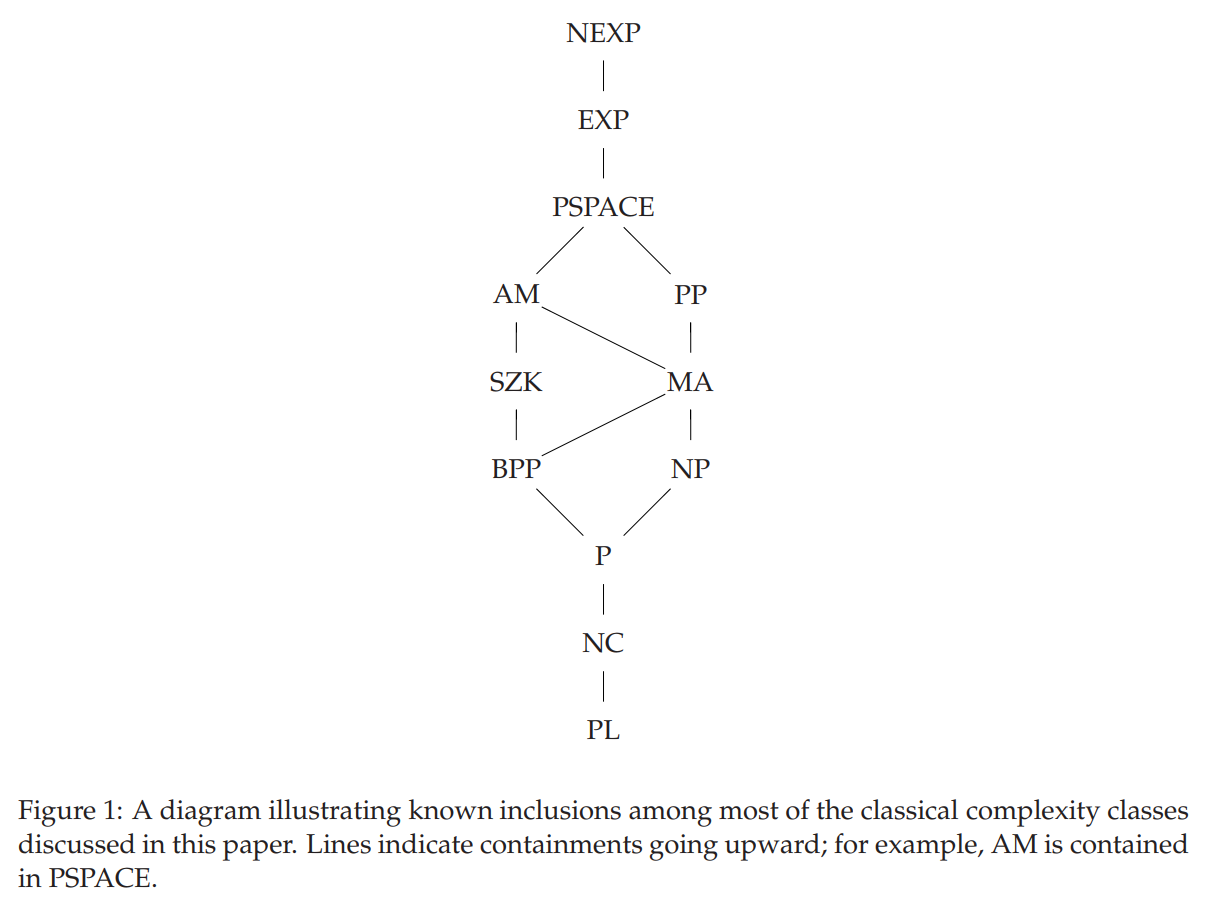
\includegraphics[scale=0.3]{complexity}
\end{figure}










\newpage






\section{Quantum Simulation: A Primer}

Here's what Feynman said in 1982:\\

\textit{``Can physics be simulated by a universal computer? [...] the physical world is quantum mechanical, and therefore the proper problem is the simulation of quantum physics [...] the full description of quantum mechanics for a large system with $R$ particles [...] has too many variables, it cannot be simulated
with a normal computer with a number of elements proportional to $R$ [ ... but it can be simulated with ] quantum computer elements. [...] Can a quantum system be probabilistically simulated by a classical (probabilistic, I'd assume) universal computer? [...] If you take the computer to be the classical kind I've described so far [..] the answer is certainly, No!''}


\subsection{Simulation in action}

The heart of simulation is the solution of differential equations which capture the physical
laws governing the dynamical behavior of a system. The goal is generally: given an initial state of the system, what is the state at some other time and/or position? Solutions are usually obtained by \textit{approximating} the state with a digital representation, then \textit{discretizing} the differential
equation in space and time such that an iterative application of a procedure carries the state from the initial to the final conditions.\\

The error in this procedure is \textit{bounded}, and known not to grow faster than some small power of the number of iterations. Furthermore, not all dynamical systems can be simulated efficiently: generally, only those systems which can be described efficiently can be simulated efficiently.\\

Simulating quantum systems using classical computers is usually inefficient. The dynamical behavior of many simple quantum systems is governed the SE:
\begin{align}
i\hbar \p_t \ket{\psi} = \had \ket{\psi}.
\end{align}
We will set $\hbar =1$.  For real particles in space, we often have
\begin{align}
i\p_t \psi(x) = \lb -\f{1}{2m}\p_x^2 + V(x) \rb \psi(x).
\end{align}

The key challenge in simulating quantum systems is the \textit{exponential} number of differential equations which must be solved. For 1 qubit evolving according to the
SE, a system of 2 differential equations must be solved; for 2
qubits, 4 equations; and for $n$ qubits, $2^n$ equations. Sometimes, insightful approximations can be made which reduce the effective number of equations involved, but there are many physically interesting quantum systems for which no such approximations are known.
\\

There are many important quantum systems for which classical simulation is intractable. For example:
\begin{align}
\mbox{Hubbard model: } \had = \sum^n_{k=1}V_0 n_{k^\uparrow}n_{k\downarrow} + \sum_{k,j\mbox{ neighbors,}\sigma} t_0 c_{k\sigma}^* c_{j\sigma}.
\end{align}
\begin{align}
\mbox{Ising mode: } \had = \sum_{k=1}^n \vec{\sigma_k}\cdot \vec{\sigma}_{k+1} .
\end{align}
Quantum computers can efficiently simulate quantum systems for which there is no known efficient classical simulation.












\subsection{The quantum simulation algorithm}

The quantum simulation is concerned with the solution of $i \p_t \ket{\psi} = \had \ket{\psi}$, which, for a time-independent $\had$, is just
\begin{align}
\ket{\psi(t)} = e^{-i\had t}\ket{\psi(0)}.
\end{align}
$\had$ is in general difficult to exponentiate, but a good beginning is the first order solution 
\begin{align}
\ket{(\psi(t+\Delta t))} \approx (\Id - i\had \Delta t)\ket{\psi(t)}.
\end{align}
This is tractable, but often is not very satisfactory. \\

Efficient approximations to higher oder is possible for many \textit{classes} of Hamiltonians. For example, in most physical systems, the Hamiltonian can be written as a sum over many \textit{local} interactions. For a system of $n$ particles:
\begin{align}
\had = \sum^L_{k=1}\had_k \sim \bigoplus^L_{k=1}\had_k
\end{align} 
where each $\had_k$ acts on at most a constant $c$ number of systems, and $L$ is a polynomial in $n$. For instance, the terms $\had_k$ are often just 2-body interactions such as $X_i X_j$ and 1-boy Hamiltonians such as $X_i$. Note that both the Hubbard and Ising models have Hamiltonians of this form. There are sometimes additional global symmetry constraints such as particle statistics.\\

Note that although $e^{-i\had t}$ is difficult to compute, $e^{-i\had_k t}$ acts on a much smaller subsystem, and is straightforward to approximate using quantum circuits. However, because $[\had_j, \had_k] \neq 0$ in general (obviously, they don't commute in general), $e^{-i\had t} \neq \prod_k e^{-i \had_k t}$. So, we might want to ask how $e^{-i\had_k t}$ be useful in constructing $e^{-i\had t}$. \\

\textbf{Remarks:}
\begin{itemize}
	\item If the $\had_i$'s commute, then we do have $e^{-i \had t} = \prod_k e^{-i \had_k t}$. 
	
	\item The restriction of $\had_k$ to involve at most $c$ particles \textit{implies} that in the sum of the Hamiltonians, $L$ is upper bounded by a polynomial in $n$. 
\end{itemize}



The heart of quantum simulation algorithms is the following asymptotic approximation theorem:
\begin{thm}[Trotter formula]
	Let $A$ and $B$ be Hermitian operators. Then for any real $t$, 
	\begin{align}
	\lim_{n\to \infty}\lp e^{-iAt/n}e^{iBt/n} \rp^n = e^{i(A+B)t}.
	\end{align}\qed
\end{thm}



Of course, the theorem holds even if $A$ and $B$ don't commute. For now, we only consider the cases where $A,B$ are Hermitian. But $A,B$ can actually be generators of certain kinds of semigroups, which correspond to general quantum operations.\\

Using the theorem (and the proof of the theorem, which I won't show here), we can get
\begin{align}
e^{i(A+B)\Delta t} = e^{iA \Delta t}e^{i B\Delta t} + \mathcal{O}(\Delta t^2).
\end{align}
Similarly, 
\begin{align}
e^{i(A+B)\Delta t} = e^{iA\Delta t/2}e^{iB \Delta t}e^{iA \Delta t/2} + \mathcal{O}(\Delta t^3). 
\end{align}







\begin{exmp}[Hamiltonian simulation \& Trotterization, taken from \href{https://vtomole.com/blog/2019/04/07/trotter}{\underline{here}} ]
	
	The evolution of quantum system is governed by the SE $i \p_t \ket{\psi} = \had \ket{\psi}$. The solution to the SE:
	\begin{align}
	\ket{\psi(t)} = e^{-i \had t}\ket{0}
	\end{align}
	is a description on what state a system will be in after a Hamiltonian has been applied to it for a certain period of time. The problem of Hamiltonian simulation is thus states as: given a Hamiltonian $\had$ and an evolution time $t$, \textbf{output a sequence of computational gates} that implement $\U = e^{-i \had t}$.\\
	
	Hamiltonians are Hermitian operators that are usually a sum of a large number of individual Hamiltonians $\had_j$. For example, $\had = H_1 + H_2$. This sum of 2 Hamiltonians (which don't necessarily commute) can be described by the Trotter formula or the Lie product formula:
	\begin{align}
	e^{-i(H_1 + H_2)t} = \lim_{N\to \infty}\lp e^{-i H_1 t/N}e^{-iH_2 t/N} \rp^N.
	\end{align}
	Since the limit of this formula is infinite, we have to truncate the series when implementing this formula on a quantum compute. The truncation introduces error in the simulation that we can bound by $\epsilon$ such that $\norm{e^{-i \had t} - \U} \leq \epsilon$, where $\norm{\cdot}$ is some operator norm. This truncation is known as \textbf{Trotterization} and it's widely used to simulate non-commuting Hamiltonians on quantum computers. The \textbf{Trotterization formula} is then
	\begin{align}
	e^{-i \had t} = \lp e^{-iH_0 t/r}e^{-i H_1 t/r} \dots e^{-iH_{d-1}t/r}  \rp^r + \mathcal{O}(\text{polynomial factors}).
	\end{align} 
	Consider for example the Hamiltonian
	\begin{align}
	\had = X_0 + Y_1 + Z_2
	\end{align}
	where $X,Y,Z$ are Pauli matrices and the subscripts label  the qubits that the Hamiltonians act on. We can't simulate each Hamiltonian separately because they don't commute. This is why we use Trotterization where we evolve the entire Hamiltonian via repeatedly switching between evolving $X_0, Y_1, Z_2$ each for a small period of time.\\
	
	The first step in deriving the circuit that will simulate this Hamiltonian is finding the quantum gates that implement each of its individual term (so that we can make $\ket{\psi(t)}= e^{-i\had t}\ket{0}$ from $\ket{0}$ -- in a sense we want to find the correct form for $e^{f(X_0)}$). It turns out that this is easy since the quantum gates
	\begin{align}
	R_x(\theta) = e^{-i\theta X/2}, \quad R_y(\theta) = e^{-i\theta Y/2}, \quad R_z(\theta) = e^{-i\theta Z/2}
	\end{align} 
	will implies the individual terms perfectly. $\theta$ here denotes an \textbf{angle}, but we can also think of it as \textbf{time} because $\theta$ specifies the angle by which to rotate the state in a specified axis, which is synonymous with time in the sense that it specifies how ``long'' the rotation is applied on the state. \\
	
	
	Since we don't care too much about the simulation error in this example we will use  $r=2, t=1$ in the Trotter formula to get
	\begin{align}
	e^{-i(X_0 + Y_1 + Z_2)} = \lp e^{-iX_0/2}e^{-iY_1/2}e^{-iZ_2/2}\rp\lp e^{-iX_0/2}e^{-iY_1/2}e^{-iZ_2/2}  \rp
	\end{align}
\end{exmp}















\subsection{The algorithm}

\begin{itemize}
	\item \textbf{Inputs:} (1) A Hamiltonian $\had = \sum_k \had_k$ acting on an $N$-dimensional system, where each $\had_k$ acts on a small subsystem of size independent of $N$, (2) an initial state $\ket{\psi_0}$, of the system at $t=0$, (3) a positive, non-zero accuracy $\delta$, and (3) a time $t_f$ at which the evolved state is desired. 
	
	
	\item A state $\ket{\tilde{\psi}(t_f)}$ such that
	\begin{align}
	\abs{\bra{\tilde\psi (t_f)} e^{-i \had t_f} \ket{\psi_0}}^2 \geq 1 - \delta.
	\end{align}
	
	
	\item Choose a representation such that the state $\ket{\tilde\psi}$ of $n = \mbox{poly}(\log N)$ qubits approximates the system and the operators $e^{- \had_k \Delta t}$ have efficient quantum circuit approximations. Selection an approximation method and $\Delta t$ such that the expected error is acceptable, construct the corresponding quantum circuit $\U_{\Delta t}$ fo the iterative step, and do the following:
	\begin{itemize}
		\item Initialize state: $\ket{\tilde \psi_0} \leftarrow \ket{\psi_0}; j = 0.$ 
		\item Iterative update: $\to \ket{\tilde \psi_{j+1}} = \U_{\Delta t}\ket{\tilde \psi_j}$.
		\item Loop: $\to j = j+1;$ go to the second step until $j\Delta t \geq t_f$.
		
		\item Final result: $\to \ket{\tilde \psi(t_f)} = \ket{\tilde \psi}$.
	\end{itemize}
\end{itemize}


\begin{thm}[Baker-Campbell-Hausdorf formula]
	\begin{align}
	e^{(A+B)\Delta t} = e^{A \Delta t}e^{B \Delta t}e^{-(1/2)[A,B]\Delta t^2} + \mathcal{O}(\Delta t^3). 
	\end{align}
\end{thm}


\begin{proof}
	The proof is quite easy. Just, by definition, expand things out in power series. \qed
\end{proof}




\subsection{An illustrative example}

We have seen the case where the Hamiltonian is a sum of local interactions. However, this is not a fundamental requirement. Efficient quantum simulations are possible even for Hamiltonians which act non-trivially on all or nearly all parts of a large system. \\

Consider the Hamiltonian
\begin{align}
\had = Z_1 \otimes Z_2 \otimes \dots \otimes Z_n
\end{align}
which acts on an $n$ qubit system. This can be simulated efficiently. What we desire is a simple quantum circuit which implements $e^{-i \had \Delta t}$, for arbitrary values of $\Delta t$. A circuit that does this is given by
\begin{figure}[!htb]
	\centering
	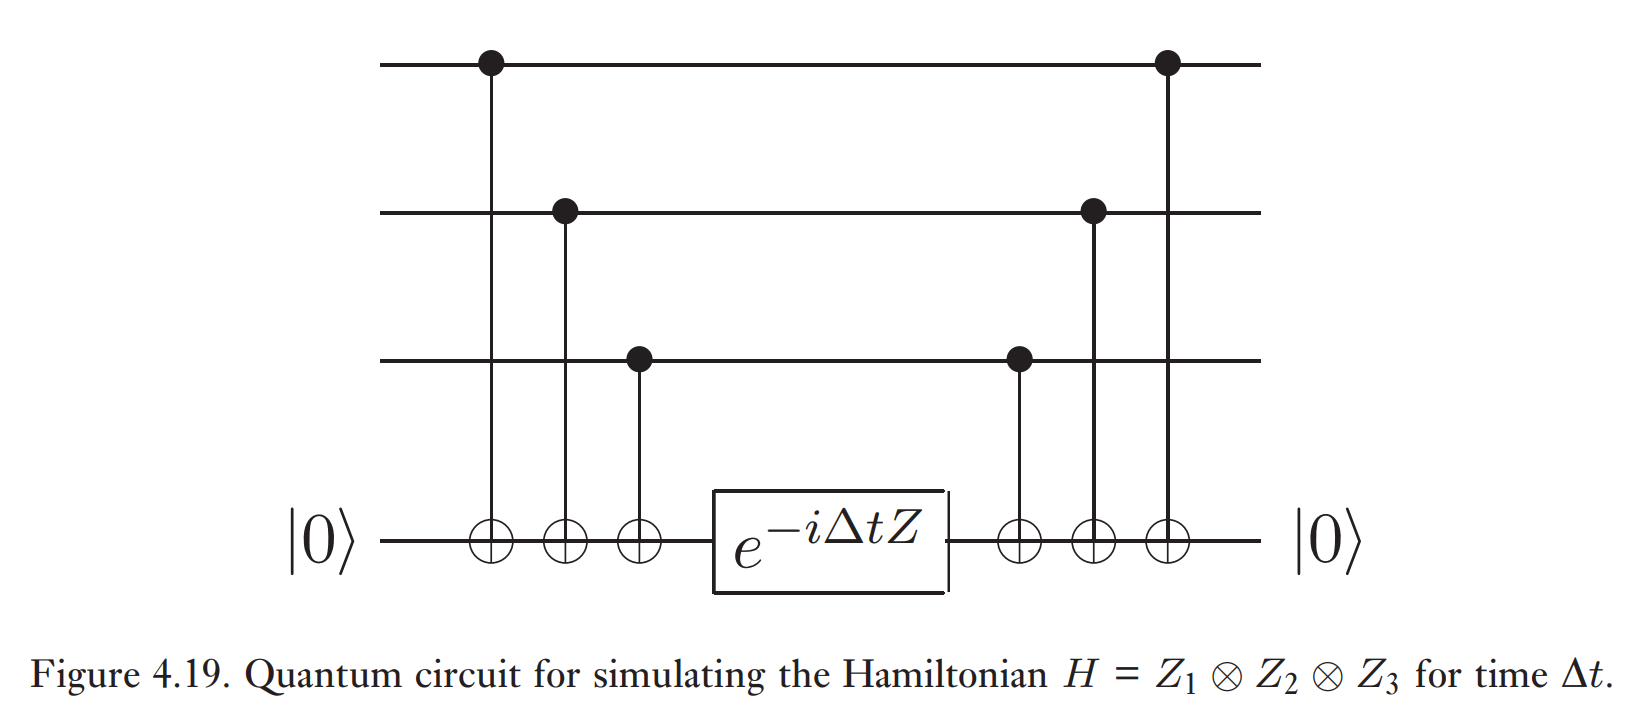
\includegraphics[scale=0.25]{qs1}
\end{figure}

Even though the Hamiltonian involves all the qubits in the system, it does so in a \textit{classical} manner: the phase shift applied to the system is $e^{-i\Delta t}$ if the \textit{parity} of the $n$ qubits in the computational basis is even. else the phase shift would be $e^{i\Delta t}$. Thus, a simple simulation of $\had$ is possible by first classical computing the parity, then applying the appropriate phase shift conditioned on the parity, then uncomputing the parity. \\

Extending the same procedure allows us to simulate more complicate extended Hamiltonians. Specifically, we can efficiently simulate any Hamiltonian of the form
\begin{align}
\had = \bigotimes^n_{k=1}\sigma^k_{c(k)}
\end{align}
where $\sigma^k_{c(k)}$ is a Pauli matrix (or identity) acting on the $k$th qubit, with $c(k) \in \{0,1,2,3\}$ specifying one of $\{I,X,Y,Z\}$. The qubits upon which the identity acts can be disregarded, and $X$ or $Y$ terms can be transformed by single qubit gates to $Z$ operations. This leaves a Hamiltonian of the form given above, which can be efficiently simulated. \\

Using this procedure allows us to simulate a wide class of Hamiltonians containing terms which are not local. It is possible to simulate a Hamiltonian of the form $\had = \sum^L_{k=1} \had_k$ where we only require that the individual $\had_k$ have a tensor product structure, and that $L$ is polynomial in the total number of particles $n$. 







\subsection{Perspectives on quantum simulation}

 
Quantum simulation is similar to classical methods, but differs fundamentally in many aspects. Each iteration of the quantum algorithm must completely replace the old state with a new one and there is no way to obtain any nontrivial information from an intermediate step without changing the algorithm (due to the no-cloning theorem). Furthermore, the final measurement must be chosen to provide the desired result because it collapses the entire state. \\

Another difficult problem is the simulation of equilibration processes. A system with Hamiltonian $\had$ in contact with an environment at temperate $T$ will come to thermal equilibrium in a state known as the \textit{Gibbs} state,
\begin{align}
\rho_{\text{therm}} = \f{e^{-\had/k_BT}}{\mathcal{Z}} \equiv \f{e^{-\had/k_BT}}{\tr\lp e^{-\had/k_BT} \rp}
\end{align}
where of course $\mathcal{Z}$ is the partition function. We can check that $\tr(\rho) = 1$. For now, we don't know how a quantum computer can simulate this. \\

Indistinguishability of particles also places a constraint on the state vector of a system which manifests itself in two ways: bosons and fermions. The state vector of a system of bosons remains unchanged under permutation of any two constituents. System of fermions experience a sign change in their state vector under interchange of any two constituents. Both kinds of systems can be simulate efficiently on a quantum computer. 















\newpage


\section{Problems in Quantum Simulations and Quantum Algorithms}

In this section, we will be looking at the following \href{https://arxiv.org/pdf/2001.03685.pdf}{\underline{review}} on quantum algorithms for quantum chemistry and materials science. 

\subsection{Quantum Simulation: An Overview}

\subsubsection{Introduction}

The interest in quantum computing for quantum simulations of molecules and materials stems from the fact that in many cases, the chemistry and physics of molecules and materials is best described using quantum mechanics. In the worst case, quantum simulation is exponentially hard on classical computers. Quantum computers have advantages over classical computers, but these advantages are problem-specific. \\


As we have seen before, the natural problem to solve on a quantum computer is the time evolution of a quantum system given some initial state:
\begin{align}
i\p_t \ket{\psi(t)} = \had \ket{\psi(t)}.
\end{align}
This problem, as we have pointed out, is of polynomial cost on a quantum computer, which can offer exponential speedup over classical computers. However, it is necessary to prepare the initial state, which may be difficult. In particular, preparing a low-energy state may be challenging, which naturally leas to considering other important problems:
\begin{align}
&\mbox{Ground state:} \quad \had\ket{\psi_0} = E_0 \ket{\psi_0}; \quad E_0 = \min_{\ket{\psi}}\bra{\psi}\had\ket{\psi}\\
&\mbox{Thermal averages:} \quad \langle \mathcal{A} \rangle = \f{\tr\lp \mathcal{A}e^{-\beta\had} \rp}{\tr\lp e^{-\beta\had} \rp}
\end{align} 
Ground state determination lies in complexity class QMA, a class of problems \textit{not known to be efficiently solvable in general on a quantum computer}. This means that thermal averages cannot in general be computed efficiently on a quantum computer, since in the limit of zero temperature, this problem reduces to ground-state determination. \\

To understand quantum advantage in chemistry, condensed matter physics, and quantum materials science, we must be guided by actual empirical data in the form of numerical and theoretical experiments with quantum algorithms and quantum devices on simulation problems of interest. This requires progress, of course. 



\subsubsection{Current quantum architectures}
There's \textit{analog quantum computation} and there's \textit{digital quantum computation}. Analog quantum computation was proposed by Feynman. The idea of analog quantum computation is to build a lattice of spins with tunable interactions and let it simulate physical systems. The limitation, however, is that this is quite limited because it can only simulate a certain set of physical systems. Furthermore, its accuracy is limited. \\

Digital quantum computation is more general. Digital quantum computation involves qubits and gates. One can show that with a finite set of gates, one can in principle generate arbitrary quantum evolutions to arbitrary precision. Every problem in the complexity class BQP can be mapped into a quantum program. \\


The third model of quantum computation is \textit{adiabatic quantum computation}. This model is considered equivalent to the digital version, but is less practical. We won't worry about this. 



\subsubsection{Building a circuit-based digital quantum computer}

The natural enemy of quantum computation is decoherence -- the tendency of quantum systems to decay into their classical states. We are current in the \textit{noisy intermediate-scale quantum} (NISQ) era, where qubit technologies (superconducting qubits, ion traps, etc) have reached the point where small devices of a few dozen qubits can be sufficiently isolated from decoherence to execute non-trivial quantum algorithms of a few tens to hundreds of gates. With these devices, an artificial but well-defined problem that is intractable classically is solved on a quantum computer. However, these problems are often not practical. The more important question is when a more relevant problem can be solved on a quantum computer. \\


To address large-scale problems, \textit{quantum error-correction} (QEC) is necessary. QEC leads to a distinction between \textit{logical} and \textit{physical} qubits. The former are error-corrected and encoded in the state of many physical qubits. Quantum algorithms are performed on the logical qubits, and the error-correction scheme translates the operations on logical qubits into physical operations. 



\newpage




\subsection{Simulation challenges in molecular and materials science }

In this section we look at some scientific problems of relevance to quantum simulation.

\subsubsection{Quantum chemistry}

Quantum chemistry is concerned with determining the low-lying eigenstates of the electronic Hamiltonian of a molecule. he eigenstates are determined for fixed sets of nuclear positions within the Born-Oppenheimer approximation. Determining the electronic energy as a function of nuclear position is key to understanding chemical reactivity, product distribution, and reaction rates.\\

Some examples of problems in quantum chemistry include
\begin{itemize}
	\item The chemistry of enzyme active sites
	\item Transition metal nanocatalysts an surface catalysts
	\item Light harvesting and the vision process
\end{itemize}

The basic metric is whether ground-states or low-energy eigenstate quantum algorithms yield more accurate energies than the best classical algorithms, for the problem sizes of interest. 

\subsubsection{Quantum molecular spectroscopy}


The theoretical goal is to compute the eigenstates of the nuclear SE. There are challenges, of course. First, the nuclear Hamiltonian is often not known, because interactions are mediated by electrons. Second, nuclear rotational and vibrational motion is often far from harmonic and not well approximate by simple mean-field theories. Third, even when the nuclear SE has been properly formulated, one faces the challenge of representing th eigenstates. \\

Some famous examples include:
\begin{itemize}
	\item Spectra of floppy molecules
	\item Hydrogen bonded clusters
\end{itemize}

There are similarities with the quantum chemistry problems, but the differences are more significant. The Hamiltonian is often more complicated because interactions are now many-body. Also, the number of states is often orders-of-magnitude greater. 


\subsubsection{Chemical quantum dynamics}

Chemical quantum dynamics if concerned with modeling time-dependent electronic and nuclear quantum effects in molecules. Some problems include:
\begin{itemize}
	\item Proton coupled electron transfer
	\item Vibrational dynamics in complex environments
	\item Plasmonic chemistry
\end{itemize}


There are multiple practical challenges. Some of this may be viewed as an issue of representation. In addition, the dynamical quantum state involves near continuum degrees of freedom, which makes discretizing the Hilbert space a challenging problem. 


\subsubsection{Correlated electronic structure in materials}

The goal here is to determine low-energy properties of materials such as Mott insulators. Some famous problems include:
\begin{itemize}
	\item High-temperature superconductivity
	\item Non-Fermi liquid behavior in heavy fermion compounds and fermionic systems near criticality
	\item Quantum fluctuations in two-dimensional systems
	\item Frustrated spin systems
\end{itemize}






%\subsubsection{Dynamical quantum effects in materials}












\newpage


\subsection{Challenges for quantum algorithms in quantum simulation}

\subsubsection{Overview of algorithms}

In this section, we look at the current status and theoretical and practical challenges to implement quantum algorithms for quantum problems. \\


The first step in a quantum simulation is to choose a \textit{representation} for the Hamiltonian and the states. We will examine the possibilities for different qubit representations, and open questions.\\

Quantum ground-state algorithms fall into different classes. QPE is a direct route to nearly exact eigenstate determination, but has been challenging to implement in the near-term era. On the other hand, \textit{variational quantum algorithms} provide the possibility to introduce approximations with adjustable circuit depth, which are determine via optimization, usually implemented in a hybrid-quantum classical loop. \\

While polynomial time algorithms for \textit{quantum time evolution} have been known for some time, algorithms with optimal asymptotic complexity as well as favorable scaling with error and low prefactors, remain an area of active research.




\subsubsection{Qubit representation of many-body systems}

To simulate many-body systems on a digital computer (either quantum or classical), the infinite-dimensional Hilbert space of a many-body system has to be truncated. The most direct route then is to define a finite set of \textit{basis functions} and then try to project the exact many-body Hamiltonian onto the chosen basis. The resulting discretized system is then expressed in terms of qubits. A choice of a good representation is important as it may affect the simulation cost dramatically. 


\begin{enumerate}
	\item \textit{Ab initio electronic structure qubit representations:}\\
	
	This concerns with the electronic structure. Consider the Hamiltonian that appears regularly in chemistry and physics
	\begin{align}
	\had = \sum^K_{i=1}-\f{1}{2}\laplacian + V(r_i) + \sum_{1\leq i<j\leq K}\f{1}{\abs{r_i - r_j}}
	\end{align}
	where $K$ is the number of electrons, $V$ is the potential created by atomic nuclei at a point $r$, and the last term represents the Coulomb interaction. Each electronic has $r_i \in \mathbb{R}^3$ and spin $\omega_i \in \{\uparrow, \downarrow\}$. So, the total wavefunction (for $K$ electrons) has the form $\psi = \psi(\vec{x}_1,\dots,\vec{x}_K)$ where $\vec{x}_i = (r_i,\omega_i)$. From Fermi statistic, we require that $\psi$ is anti-symmetric under a position swap.\\
	
	The first step is to approximate the electronic Hamiltonian with a simpler simulator Hamiltonian. This is usually achieved by truncate the Hilbert space of a single electron to a finite set of basis functions $\psi_1,\dots,\psi_N$. \\
	
	Electronic structure simulation algorithms are based on the \textit{first quantization method} (\href{https://journals.aps.org/prl/pdf/10.1103/PhysRevLett.79.2586}{\underline{link}}). We won't worry about this too much.\\
	
	The \textit{second quantization method} often results in simpler simulator Hamiltonian and requires few qubits. This methods is particularly well suited for quantum simulation algorithms and has been experimentally demonstrated for small molecules. Given a set of $N$ basis functions $\psi_1,\dots,\psi_N$, the second quantized simulator Hamiltonian is given by
	\begin{align}
	\had = \sum^N_{p,q=1} t_{pq}\hat{c}_p^\dagger \hat{c}_q + \f{1}{2}\sum^N_{p,q,r,s=1}u_{pqrs}\hat{c}^\dagger_p\hat{c}_q^\dagger \hat{c}_r \hat{c}_s.
	\end{align}
	Again, we're not going to worry too much about these. 
	
	
	
	
	
	
	
	\item \textit{Electronic basis functions:}\\
	
	The discretization of the electronic Hilbert space for a quantum simulation requires balancing two concerns. We need to represent the state with the smallest number of qubits, but also retain maximal Hamiltonian sparsity. \\
	
	There are two families of basis functions in wide use in quantum chemistry and quantum materials science: atomic orbital \textit{Gaussian bases} and \textit{Plane waves}. Gaussian bases are commonly used in molecular simulations due to their compactness, while plane waves are used in crystalline materials simulations. \\
	
	In Gaussian bases, linear combinations of Gaussian functions are placed at the nuclear positions. When they are place where the ground-state electron density is highest, they give a compact representation of the wavefunction for bound states. However, the Hamiltonian is not sparse, which leads to high gate counts. \\
	
	Plane waves offer greater simplicity as the accuracy of the basis is controlled by a single parameter, namely the kinetic energy cutoff. The number of plane waves needed to reach a desired accuracy is larger than th number of Gaussian states, but the Hamiltonian contains fewer terms ue to momentum conservation. \\
	
	The need to expose more sparsity in the Hamiltonian while retaining a reasonable compact wavefunction is an active area of research in both classical and quantum algorithms.  
	
	
	\item \textit{Fermions-to-qubit mappings:}\\
	
	Since the basic units of a quantum computer are qubits rather than fermions, any quantum simulation algorithm of fermions emplyos a suitable encoding of fermionic degrees of freedom into qubits. The standard \textit{Jordan-Wigner} mapping identifies each Fermi mode with a qubit such that the empty and the occupied states are mapped to the qubit basis states $\ket{0}$ and $\ket{1}$ respectively. The Jordan-Wigner mapping/transformation is a transformation that maps spin operators onto fermionic creation and annihilation operators. 
	\begin{figure}[!htb]
		\centering
		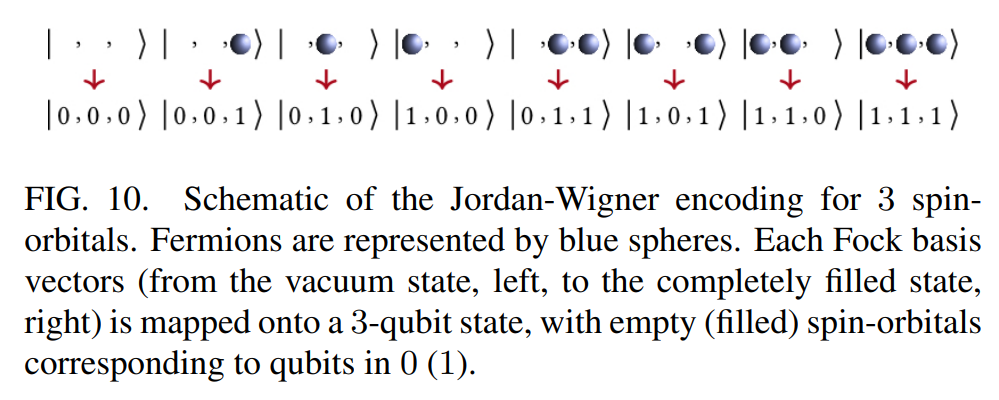
\includegraphics[scale=0.3]{jw}
	\end{figure}
	A natural question is whether the number of qubits required to express a Fermi system can be reduced by exploiting symmetries such as the particle number conservation or
	the point group symmetries of molecules. For example, zero
	temperature simulations often target only one symmetry sector containing the ground state. This motivates the study
	of \textit{symmetry-adapted fermion-to-qubit mappings}.
\end{enumerate} 



\subsubsection{Quantum algorithms for ground and excited states}

There are many approaches to obtaining ground states or
excited states on a quantum computer. State preparation
procedures attempt to construct a circuit to prepare a state
with as large as possible overlap with the desired eigenstate. One set of such procedures, which includes adiabatic state preparation and quantum imaginary time evolution, uses a prescribe evolution path. An alternative strategy is based on \textit{variational methods}, which are often called variational quantum eigensolvers. Here, the preparation circuit itself is defined via the optimization of the energy with respect to parameters of the circuit. \\


Given some state with sufficiently large overlap with the desired state, one can perform \textit{quantum phase estimation} (QPE) which simultaneously projects the state onto an eigenstate of the Hamiltonian and obtains an estimate for the energy of this eigenstate. The error, as we have seen, is inversely proportional to the simulation time. The probability of successfully projecting onto the desired state is given by the square overlap of the input state and
the desired state, and it is thus necessary to use some other
method (such as the state preparation procedures above) to
prepare an input state with sufficient overlap with the desired
state.\\


There are weaknesses to this, of course. While phase estimation allows the deviation of the final state from an exact eigenstate to be systematically reduced, it can require deep circuits with many controlled gates that are challenging for devices with limited coherence and without error correction. Variational methods replace such circuits b a large number of potentially short simulations. However, if one des not measure the energy by phase estimation, but instead by expressing the Hamiltonian as a sum of multi-qubit Pauli operators and measuring the terms individually, the state preparation and measurements must be repeated many times, with the error converging only as the square root of the number of repetitions. Variational methods are also limited by the variational form and ability to solve the associated optimization
problem, which may by itself represent a difficult classical
optimization.


\subsubsection{Preparing ground states along a prescribed path}

\begin{enumerate}
	\item \textit{Adiabatic state preparation:}\\
	
	 
	This state preparation relies on the \textit{adiabatic theorem}
	
	
	\begin{thm}[Adiabatic Theorem]
		A physical system remains in its instantaneous eigenstate if a given perturbation is acting on it slowly enough and if there is a gap between the eigenvalue and the rest of the Hamiltonian's spectrum. 
	\end{thm}
	In simpler terms, this says that gradually changing conditions allow the system to adapt its configuration, hence the probability density is modified by the process. if the system started in an eigenstate of the initial Hamiltonian, it will end in the \textit{corresponding} eigenstate of the final Hamiltonian.\\
	
	To make use of this theorem, one chooses a Hamiltonian path $\had(\lambda)$ where $\lambda \in [0,1]$, such that the ground state of $\had(0)$ is easily prepared, while $\had(1)$ is the Hamiltonian whose ground state one wants to obtain. The system is then evolved under the time-dependent SE 
	\begin{align}
	i\p_t \ket{\psi_t} = \had(t/T)\ket{\psi_t},\quad t \in [0,T].
	\end{align}
	When $T\to \infty$ and if the spectrum of $\had_{t/T}$ is gapped for all $t$, the final state is the exact ground state of $\had$. Away from the adiabatic limit $T\to \infty$, corrections are necessary. \\
	
	The main disadvantage of this approach is that it is limited by the $T\to \infty$ requirement, and the fact that a path without degeneracies must be chosen. 
	
	
	\item \textit{Quantum imaginary-time evolution:} \\
	
	In classical simulations, one popular approach to prepare (nearly exact) ground-states is imaginary-time evolution,
	which expresses the ground-state as the long-time limit of the
	imaginary-time SE $-\p_t \ket{\Phi(\beta)} = \had \ket{\Phi(\beta)}$:
	\begin{align}
	\ket{\psi} = \lim_{\beta \to \infty} \f{e^{-\beta \had} \ket{\Phi(\beta)}}{\norm{e^{-\beta \had} \Phi(\beta)}}.
	\end{align} 
	To perform imaginary time evolution on a quantum computer, it is necessary to implement the (repeated) action of the
	short-imaginary-time propagator $e^{-\Delta \tau \had}$
	on a state. Given a Hamiltonian that can be decomposed into geometrically local terms,
	\begin{align}
	\had = \sum _m \hat{h}_m
	\end{align}
	and a state $\ket{\psi}$ with finite correlation length $C$, the action $e^{-\Delta \tau \hat{h}_i}$ can be generated by a unitary $\U = e^{i\hat{A}}$ acting on $\mathcal{O}(C)$ qubits surrounding those acted on by $\hat{h}_i$, i.e.,
	\begin{align}
	\f{e^{-\beta \had} \ket{\psi}}{\norm{e^{-\beta \had} \psi}} = \U \ket{\psi}= e^{i\hat{A}}\ket{\psi}
	\end{align}	
	where the coefficients of the Pauli strings in $\hat{A}$ can be determined from local measurements of the quits around $\hat{h}_i$.\\
	
	Quantum imaginary time evolution becomes inefficient in terms of the number of measurements an complexity of the operator $\hat{A}$ if the domain $C$ grows to be large along the imaginary time evolution path. 
	
	
	
	
	
	
	
	
	
	
	
\end{enumerate}








\subsubsection{Variational state preparation and variational quantum eigensolver}


States can also be prepared through variational methods. Here, similar to classical variational approaches, one chooses a class of ansatz states for the ground state of the Hamiltonian of interest. Generally speaking, such an ansatz consists of some initial state and a unitary circuit parametrized by some set of classical variational parameters. Applying this circuit to the initial state
yields a guess for the ground state, whose energy is then evaluated. This yields an upper bound to the true ground state
energy. One then varies the variational parameters to lower
the energy of the ansatz state.\\

Choosing the class of ansatz states is also a balancing act. On the one hand, the class should contain an accurate approximation to the true ground state of the system. On the other hand, we want a class of circuits that are easily executed on the available quantum computer. Finally, it
is important for the classical optimization over the variational
parameters to be well-behaved, so as to be able to find low-energy minima. 


\begin{enumerate}
	\item \textit{Unitary coupled cluster:} \\
	
	\begin{figure}[!htb]
		\centering
		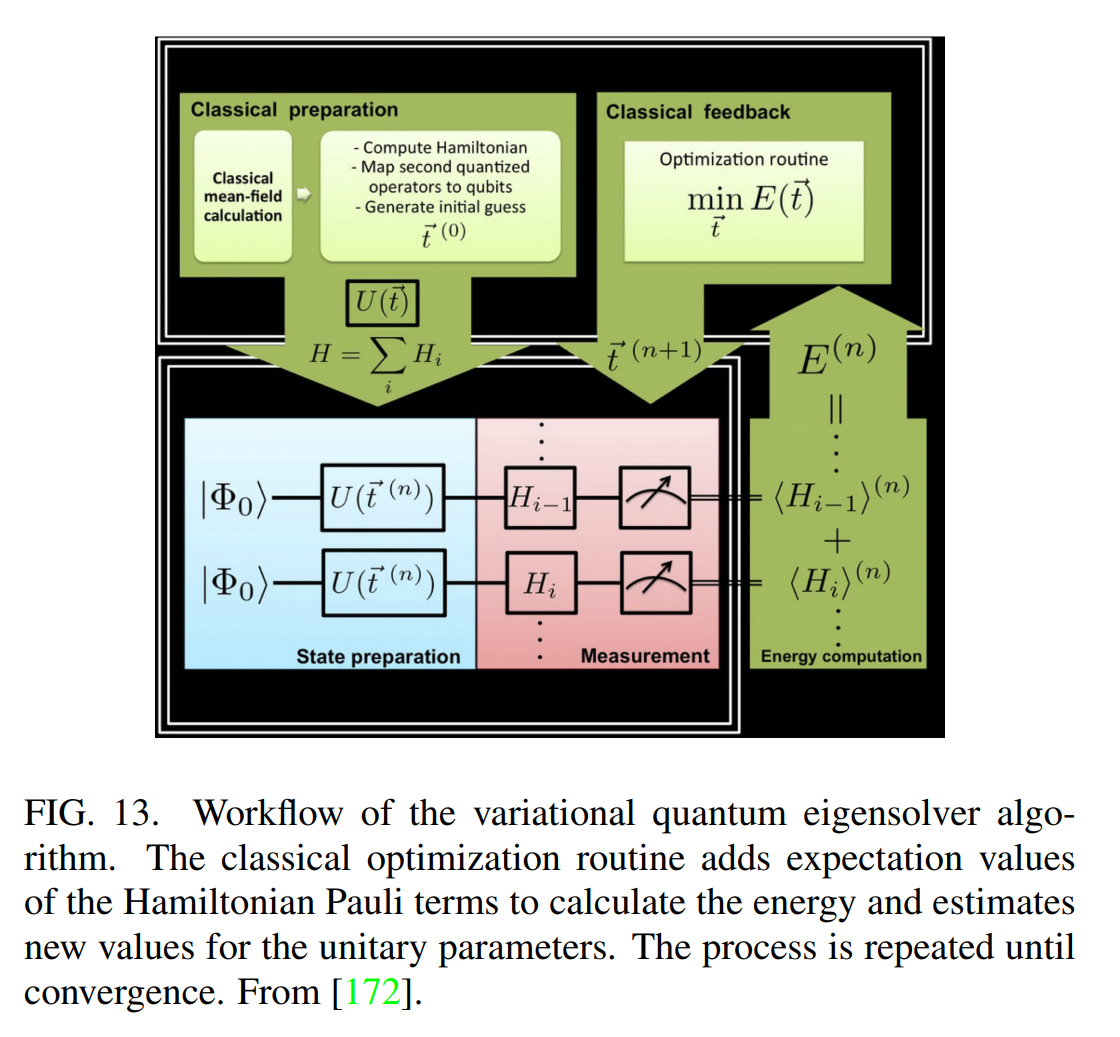
\includegraphics[scale=0.3]{vqei}
	\end{figure}
	We won't worry about the details of how this works at this point. For more information, consider this \href{https://iopscience.iop.org/article/10.1088/2058-9565/aad3e4/pdf}{\underline{paper}}.
	

	
	\item \textit{Adapt-VQE ansatz:}\\
	
	In the adapt-VQE scheme, a collection of operators $\hat{A}_i$ is chosen in advance, and the ground state is approximated by 
	\begin{align}
	\ket{\psi_{\text{adapt-VQE}}} = e^{\theta_n \hat{A}_n}\dots e^{\theta_1 \hat{A}_1}\ket{\psi_{\text{HF}}},
	\end{align}
	Given a current parameter configuration $\vec{\theta}$, the commutator  of the Hamiltonian with each operator in the pool is measured to obtain the gradient of the energy
	\begin{align}
	E = \bra{\psi_{\text{adapt-VQE}}} \had \ket{\psi_{\text{adapt-VQE}}}.
	\end{align}
	wrt the parameters $\vec{\theta}$. Repeating this multiple times and averaging over the obtained samples gives the gradient of the expectation value of the Hamiltonian wrt to the coefficient of each operator. The ansatz is improved by adding the operator $\hat{A}_i$ with the largest gradient to the left end of the ansatz with a new variational parameter, thereby increasing $n$. The operation is repeated until convergence.  
	
	
	
	
	\item \textit{Other considerations:}\\
	
	 There are other considerations with regards to variational methods, but we won't worry about them too much for now.
\end{enumerate}






\subsubsection{Excited states}

While much of the above discussion of state preparation
and variational algorithms has focused on ground-states, most
of the same methods can also be used with minor extensions
for excited states. For example, adiabatic state preparation can
be used to prepare an excited state, so long as it is connected
to the initial state without a vanishing gap.


\subsubsection{Phase estimation}

We have a section on this, so let's just be brief and gloss over the details. \\


Quantum Phase Estimation (QPE) is a crucial step in many
quantum algorithms. QPE enables high-precision measurements of the ground and excited energy levels. This is done by preparing a trial initial state $\ket{\psi(0)}$ that has a non-negligible overlap with the relevant eigenvector of the target Hamiltonian $\had$ and applying a circuit that creates a superposition of time evolved states $\ket{\psi(t)} = e^{-i\had t}\ket{\psi(0)}$ over a suitable range of evolution times $t$. \\

Since QPE is used ubiquitously in a variety of quantum applications, it is crucial to optimize its performance. Below we
list some open problems that are being actively investigated:
\begin{itemize}
	\item Given limitations of near-term quantum devices, of particular interest are tradeoffs between the depth of the
	QPE circuit and its spectral-resolution power as well
	as its sensitivity to noise.
	
	\item Several methods have been proposed for mitigating experimental errors for VQE-type simulations. Such methods enable reliable estimation of expected values of observables on a given trial state without introducing any overhead in terms of extra qubits or quantum gates.
	
	
	\item Classical post-processing methods that enable simultaneous estimation of multiple eigenvalues are highly desirable.
	
	\item Finally, a natural question is whether the time evolution
	operator $e^{-i \had t}$
	in QPE can be replaced by some other
	functions of Hˆ that are easier to implement
\end{itemize}




\subsubsection{Quantum algorithms for time evolution}


\begin{enumerate}
	\item \textit{Hamiltonian simulation problem:}  \\
	
	A quantum computer can be programmed to efficiently simulate the unitary time evolution of almost any physically realistic quantum system. Consider any evolution which is of course given by the SE
	\begin{align}
	i \p_t \ket{\psi(t)} = \had \ket{\psi(t)}, \quad t \geq 0.
	\end{align}
	We can just assume that $\had$ describes a system of $n$ qubits, since any fermionic or spin system can be mapped to qubits. Integrating we get
	\begin{align}
	\ket{\psi(t)} = e^{-i\hat t}\ket{\psi(0)}.
	\end{align}
	A quantum algorithm for Hamiltonian simulation takes as input a description of $\had$, the evolution time $t$, nd outputs a quantum circuit $\U$ that approximates the time evolution operator $e^{-it\had}$ within a specified precision $\epsilon$:
	\begin{align}
	\norm{\U - e^{-it\had}} \leq \epsilon.
	\end{align}
	$\U$ may use ancillary qubits initialized in the $\ket{0}$ state. The simulation cost is usually quantified by the runtime of the algorithm (gate count) and the total number of qubits. Applying $\U$ to $\ket{\psi(0)}$ gives the approximation state $\ket{\psi(t)}$. \\
	
	
	Quantum simulation algorithms apply to general classes of Hamiltonians satisfying mild technical conditions that enable a quantum algorithm to access the Hamiltonian efficiently.

\end{enumerate}

















%\subsubsection{Algorithmic tools}
%\subsubsection{Open problems}
%\subsubsection{Finite-temperature algorithms}
%\subsubsection{Hybrid quantum-classical methods}
%\newpage
%
%
%\subsection{Reading out results}
%
%\subsubsection{Equal-time measurements}
%\subsubsection{Dynamical properties and Green's functions}






\newpage






\section{Quantum Phase Estimation (QPE)}

One of the most important applications of the Quantum Fourier Transform is the Quantum Phase Estimation. Phase estimation is the key for many quantum algorithms. Suppose a unitary operator $\U$ has an eigenvector $\ket{u}$ with eigenvalue $2^{2\pi i \varphi}$, where the value of $\varphi$ is unknown. The goal of the phase estimation algorithm is to estimate $0 \leq \varphi \leq 1$ with high probability within additive error $\epsilon$. The algorithm uses $\mathcal{O}(\log (1/\epsilon))$ qubits and $\mathcal{O}(1/\epsilon)$ controlled-$\U$ operations. \\

To perform the estimation we assume that we have available \textit{oracles} capable of preparing the state $\ket{u}$ (the eigenstate) and performing the controlled-$\U^{2j}$ operation, for suitable nonnegative integers $j$. Since preparing eigenstates is not necessarily easy, the phase estimation algorithm is not a complete algorithm by itself. Rather, we should view it as a ``subroutine'' or a ``module.''\\



The QPE uses two registers. The first register contains $t$ qubits initially in $\ket{0}$. The choice of $t$ depends on two things: the number of digits of accuracy we wish to have in our estimate of $\varphi$, and with what probability we wish the phase estimation procedure to be successful. The second register begins in the eigenstate $\ket{u}$, and contains as many qubits as necessary to store $\ket{u}$. \\

QPE occurs in two main stages. First, the circuit applies  an $\had$ to each of the $t$ qubits. Then, the circuit applies controlled-$\U$ operators on the second register, with $\U$ raised to successive powers of two. This stage looks like the following:
\begin{figure}[!htb]
	\centering
	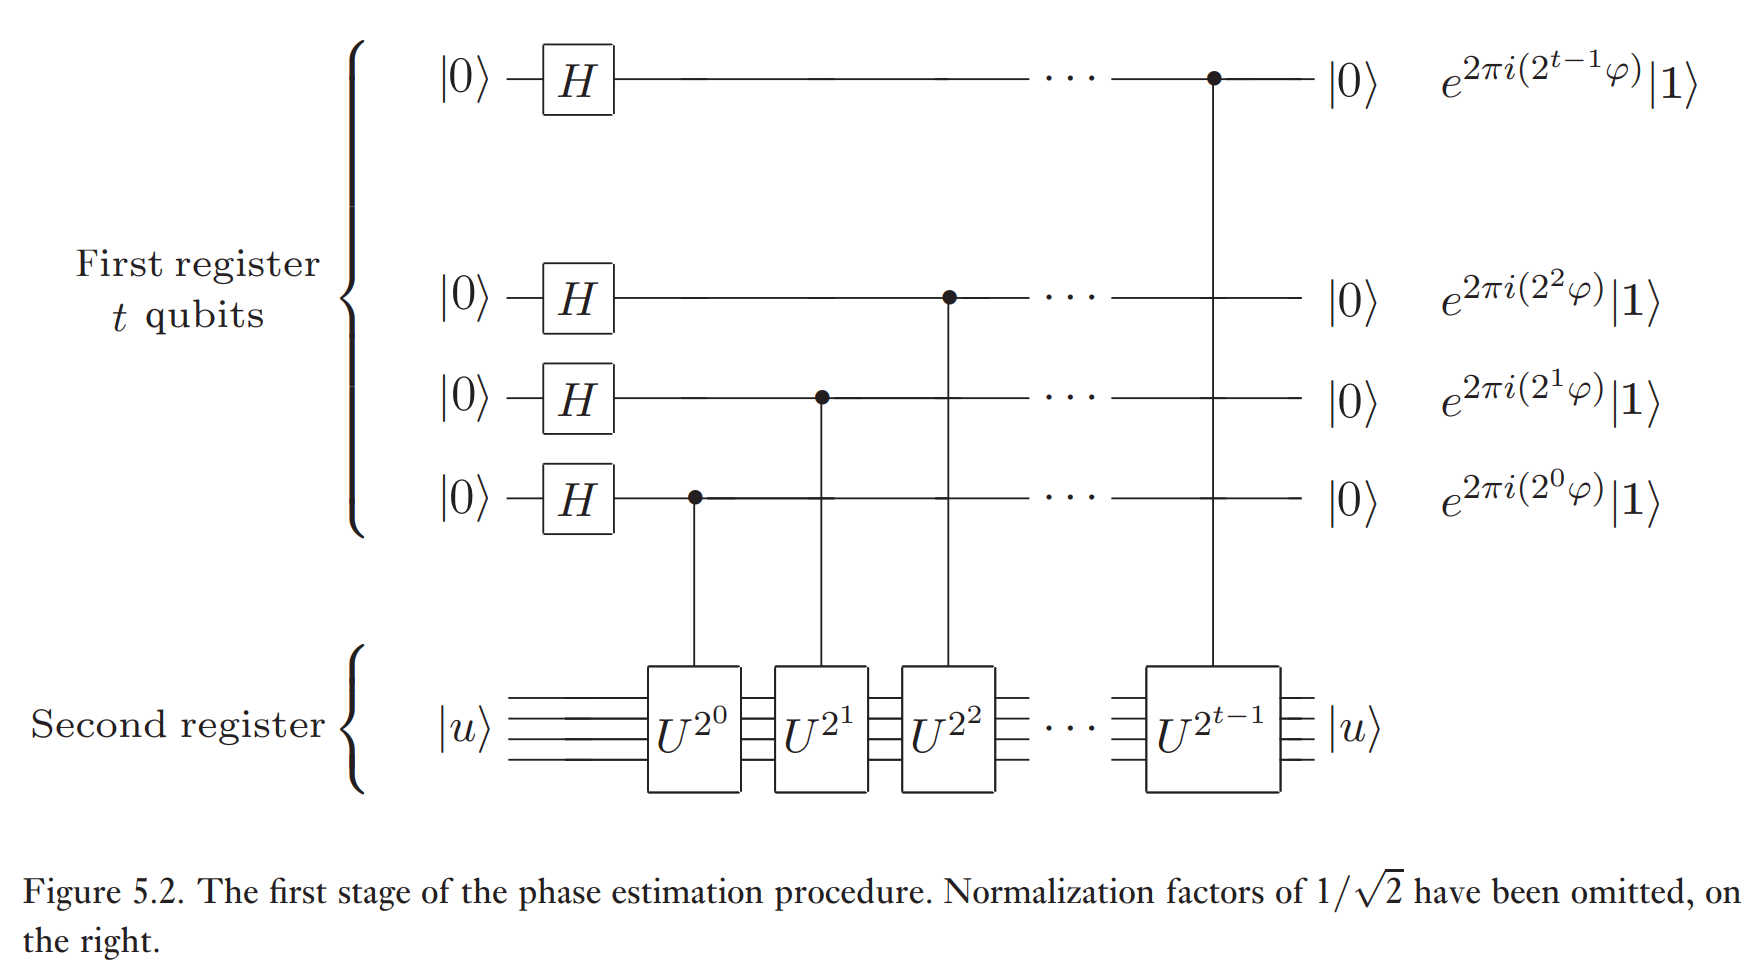
\includegraphics[scale=0.25]{qpe1}
	\caption{Source: Mike and Ike}
\end{figure} 
Recall that immediately after $\had^{\otimes t}$ the state of the upper register looks like
\begin{align}
\had \ket{0} = \f{1}{2^{1/2}}\lp \ket{0} + \ket{1} \rp
\end{align}
The controlled-$\U$ acts on $\ket{u}$ only if the control qubit is in $\ket{1}$. With this, we see that the final state of the first register is given by
\begin{align}
&\f{1}{2^{t/2}}\lp \ket{0} + e^{2\pi i 2^{t-1}\varphi}\ket{1} \rp\otimes
\lp \ket{0} + e^{2\pi i 2^{t-2}\varphi}\ket{1} \rp \otimes \dots \otimes \lp \ket{0} + e^{2\pi i 2^{0}\varphi}\ket{1} \rp\nn\\
&\quad = \dots \nn\\
&\quad = \f{1}{2^{t/2}}\sum_{0\leq k < 2^{t}} e^{2\pi i \varphi k}\ket{k}_t.
\end{align}

\begin{exmp}
For $t =2$, we have
\begin{align}
&\f{1}{2}\lp \ket{0} + e^{4\pi i \varphi } \ket{1} \rp\otimes \lp \ket{0} + e^{2\pi i\varphi }\ket{1} \rp \nn\\
&\quad= \f{1}{2}\lp \ket{0}_2 + e^{1\cdot 2\pi i\varphi }\ket{1}_2 + e^{2\cdot 2\pi i\varphi}\ket{2}_2 + e^{3\cdot 2\pi i\varphi }\ket{3}_2  \rp\nn\\
&\quad = \f{1}{2^{2/2}}\sum_{0 \leq k < 2^{2}}e^{2\pi i \varphi \cdot 2}\ket{k}_2
\end{align}\qed
\end{exmp}

Note that we're leaving out the qubits carrying the  $\ket{u}$ state because we don't do anything to it (because $\ket{u}$ is an eigenstate of $\U$). We should also note that the effect of the sequence of controlled-$\U$ operations is to take $\ket{j}\ket{u}$ to $\ket{j}\U^j \ket{u}$. We should also note that this does not depend on the fact that $\ket{u}$ is an eigenstate of $\U$. \\


In the second state, the algorithm applies the inverse quantum Fourier transform on the first register (which is just the QFT, applied in reverse order of operations). This can be done efficiently in $\mathcal{O}(t^2)$ steps, as we have seen the Quantum Information \href{https://huanqbui.com/LaTeX 20projects/HuanBui_QI/HuanBui_QI.pdf}{\underline{notes}}. Since the input in this case is the maximal superposition in the $t$-vector space, the output of the inverse QFT is going to be a single state: $\ket{\tilde{\varphi}}$, which we hope is approximately $\ket{\varphi}$. We will see how close $\ket{\tilde\varphi}$ can get to $\ket{\varphi}$.\\

The third and final stage of the algorithm is to read out the state of the first register by doing a measurement in the computational basis. \\


\begin{exmp}
	To make sure we see what is going on, suppose $\varphi$ is expressed exactly in $t$ qubits, as $\varphi = 0,\varphi_1\varphi-2\dots\varphi_t$ (note that $\varphi \in [0,1]$). Then the state of the input register after the first stage is given by
	\begin{align}
	\f{1}{2^{t/2}}\lp \ket{0} + e^{2\pi i 0.\varphi_t} \ket{1} \rp \otimes \lp \ket{0} + e^{2\pi i 0.\varphi_{t-1}\varphi_t}\ket{1} \rp \otimes \dots  \otimes \lp \ket{0} + e^{2\pi i 0.\varphi_1\varphi_2\dots\varphi_t}\ket{1} \rp.
	\end{align}
	Applying the inverse QFT to this, we see that output state from the second state is the product state $\ket{\varphi_1\dots \varphi_t}$. A measurement in the computational basis gives $\varphi$ exactly. \qed
\end{exmp}

Schematically, the algorithm for QPE looks like the following:
\begin{figure}[!htb]
	\centering
	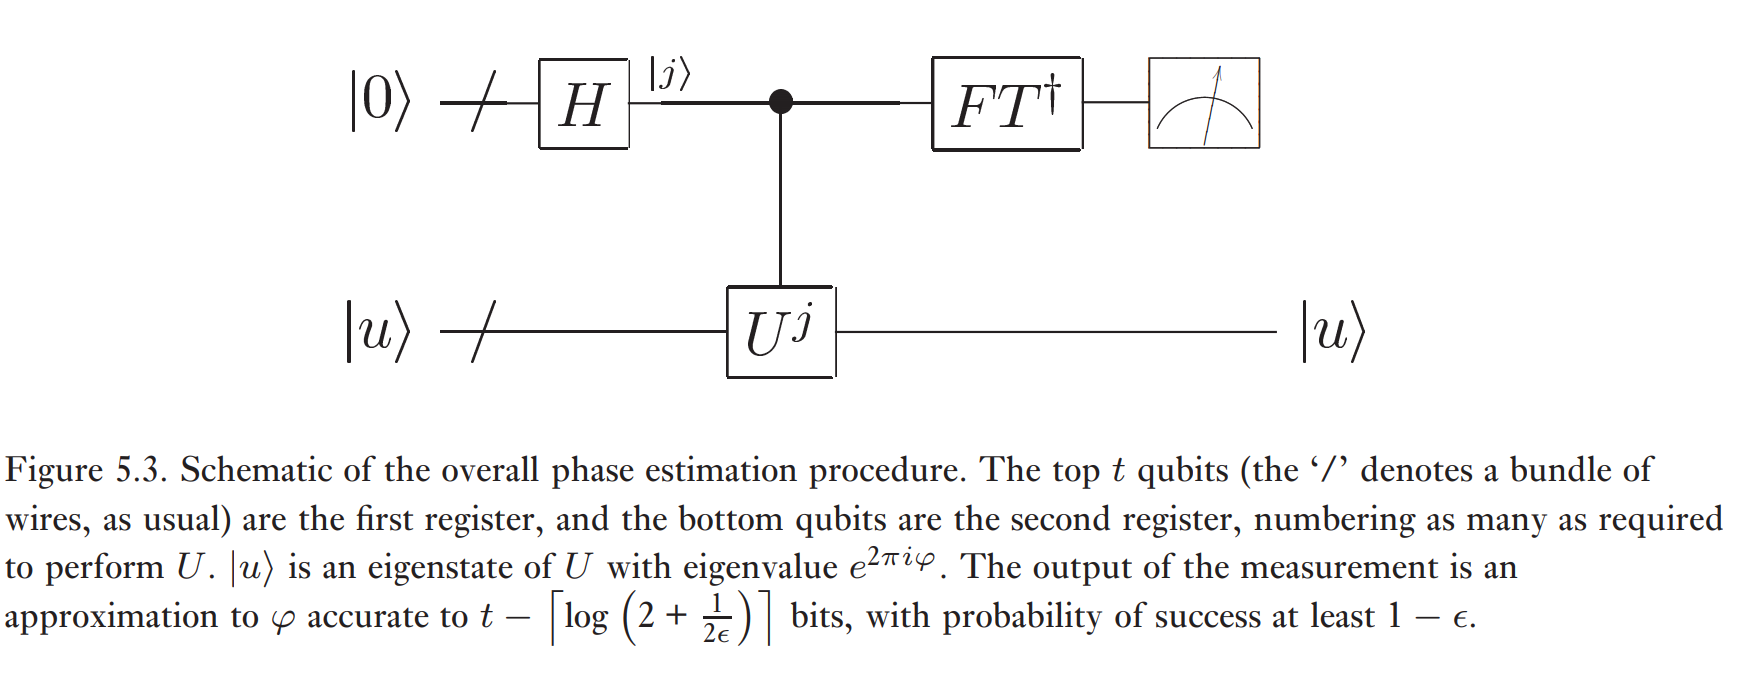
\includegraphics[scale=0.25]{qpe2}
	\caption{Source: Mike and Ike}
\end{figure}

In summary, what we basically did was using the inverse QFT to get
\begin{align}
\f{1}{2^{t/2}}\sum_{0 \leq k < 2^{t}} e^{2\pi i \varphi j }\ket{j}\ket{u} \to \ket{\tilde{\varphi}}\ket{u}
\end{align}
where $\ket{\tilde\varphi}$ is a good estimator for $\varphi$ when measured. 

 





\subsection{Performance and Requirements}
What happens when $\varphi$ cannot be written exactly with a $t$-bit expansion? We will now show that the procedure we described will produce a good approximation to $\varphi$ with high probability. \\

Let $b \in [0,2^t-1]$ an integer be given such that $b/2^t = 0.b_1b_2\dotsb_t$ is the best $t$ bit approximation to $\varphi$ which is less than $\varphi$, i.e., 
\begin{align}
0 \leq \delta \equiv \varphi - b/2^t \leq 2^{-t}.
\end{align}
(This is getting pretty close to an analysis proof -- because it \textit{is} an analysis proof.) Applying the inverse QFT to the state immediately after the first stage gives
\begin{align}
\mathcal{F}^{-1}\lb\f{1}{2^{t/2}}\sum_{0 \leq k < 2^t}e^{2\pi i \varphi k}\ket{k} \rb &= \f{1}{2^{t}} \sum_{0 \leq k,l < 2^t} e^{\f{-2\pi i kl}{2^t}}e^{2\pi i \varphi k}\ket{l}\nn\\
& = \f{1}{2^t}\sum_{0 \leq k,l < 2^t}\lp e^{2\pi i(\varphi- l/2^t)} \rp^k \ket{l}
\end{align}
by definition. Note that when $\varphi$ can be expressed using exactly $t$ bits we are reduced to the simpler version of the problem described above. \\

Let $\al_l$ be the amplitude of $\ket{(b+l) \mod 2^t}$, i.e., 
\begin{align}
\alpha_l \equiv \f{1}{2^t}\sum_{0 \leq k < 2^t} \lp e^{2\pi i (\varphi - (b+l)/2^t)} \rp^k.
\end{align}
This is a partial sum of a geometric series. It is straightforward to show that
\begin{align}
\alpha_l = \f{1}{2^t}\lp \f{1 - e^{2\pi i (2^t \varphi - (b+l))}}{1 - e^{2\pi i (\varphi - (b+l)/2^t)}} \rp = \f{1}{2^t}\lp \f{1 - e^{2\pi i (2^t \delta - l)}}{1 - e^{2\pi i (\delta - l/2^t)}} \rp.
\end{align}
Suppose the outcome of the final measurement is $m$. We want to bound the probability that $\abs{m-b} > \epsilon$ (where $\epsilon$ is the tolerance), i.e., we don't want the probably that $m$ is far from $b$ to be large. Well, the probability of observing such an $m$ is given by
\begin{align}
P(\abs{m-b} > \epsilon) = \sum_{-2^{t-1} < l \leq -(\epsilon+1)} \abs{\al_l}^2 + \sum_{e+1 \leq l \leq 2^{t-1}}\abs{\al_l}^2.
\end{align}
For any real $\theta$, we have $\abs{1 - \exp(i\theta)} \leq 2$, so 
\begin{align}
\abs{\al_l} \leq \f{2}{2^t \abs{1 - e^{2\pi i (\delta - l/2^)}}}.
\end{align}
Further, provided $-\pi \leq \theta \leq \pi$, we have $\abs{1 - \exp(i\theta)} \geq 2\abs{\theta}/\pi$. Also, when $-2^{t-1} < l \leq 2^{t-1}$ we have $-\pi \leq 2\pi (\delta - l/2^t) \leq \pi$, so we have
\begin{align}
\abs{\al_l} \leq \f{1}{2^{t+1}(\delta - l/2^t)}.
\end{align}
With this we have
\begin{align}
p(\abs{m-b} > \epsilon) &\leq \f{1}{4}\lp \sum_{l = -2^{t-1}+1}^{-(\epsilon+1)} \f{1}{(l - 2^t \delta)^2} + \sum^{2^{t-1}}_{l = \epsilon+1} \f{1}{(l - 2^t \delta)^2}  \rp\nn\\
&\leq \f{1}{4}\lp \sum_{l = -2^{t-1}+1}^{-(\epsilon+1)} \f{1}{(l - 1)^2} + \sum^{2^{t-1}}_{l = \epsilon+1} \f{1}{(l - 1)^2}   \rp, \quad 0 \leq 2^t\delta < 1\nn\\
&\leq \f{1}{2}\sum^{2^{t-1}-1}_{l=\epsilon} \f{1}{l^2}\nn\\
&\leq \f{1}{2}\int^{2^{t-1}-1}_{\epsilon-1} \f{1}{l^2}\,dl\nn\\
&= \f{1}{2(\epsilon-1)}.
\end{align}
Suppose we wish to approximate $\varphi$ to an accuracy $2^{-n}$, i.e., we choose $\epsilon = 2^{t-n}-1$. By using $t =n+p$ qubits, we see that the probability of obtaining an approximation correct to this accuracy is at least 
\begin{align}
1-\f{1}{2(\epsilon-1)} = 1 - \f{1}{2(2^p - 2)}.
\end{align}
So, to successfully obtain $\varphi$ accurate to $n$ bits with probability of success at least $1-\epsilon$ we choose 
\begin{align}
t = n + \left\lceil \log \lp 2 + \f{1}{2\epsilon} \rp \right\rceil.
\end{align}

Now here's a catch: to use QPE, we need the eigenstate $\ket{u}$. What if we don't know how to prepare such a state? Suppose that we prepare some other state $\ket{\psi}$ in place of $\ket{u}$. We can write
\begin{align}
\ket{\psi} = \sum_u c_u \ket{u}
\end{align}
where $\ket{u}$ are the eigenstates of $U$. Suppose the eigenstate $\ket{u}$ has the eigenvalue $e^{2\pi i \varphi_u}$. Running the QPE on $\ket{\psi}$ will give
\begin{align}
\ket{\psi} \stackrel{\mbox{QPE}}{\to} \sum_u c_u \ket{\tilde{\varphi_u}}\ket{u},
\end{align}
where $\tilde{\varphi_u}$ is an estimation for $\varphi_u$. Reading out the first register gives us a good approximation for $\varphi_u$, where $u$ is chosen at random with probability $\abs{c_n}^2$. This procedure allows us to avoid preparing a possibly unknown eigenstate, but at the cost of introducing some additional randomness into the algorithm. It turns out that if $t$ is chosen according to the minimization procedure above, then the probability for measuring $\varphi_u$ accurate to $n$ bits at the conclusion of the phase estimation algorithm is at least $\abs{c_u}^2(1-\epsilon)$.







\subsection{The algorithm}
QPE solves a problem which is both non-trivial and interesting from a physical point of view. It allows us to estimate the eigenvalue associated to a given eigenvector of a unitary operator. It turns our that other interesting problems can be reduced to phase estimation, which makes QPE particularly useful.\\

\underline{Here's the algorithm:}
\begin{itemize}
	\item \textbf{Inputs:} (1) An oracle which performs a controlled-$\U^j$ operation, (2) an eigenstate $\ket{u}$ of $\U$ with eigenvalue $e^{2\pi i \varphi_u}$, and (3) $t = n + \left\lceil \log \lp 2 + 1/2\epsilon \rp \right \rceil$ qubits initialized to $\ket{0}$.
	
	
	\item \textbf{Outputs:} An $n$-bit approximation $\tilde\varphi_u$ of $\varphi_u$. 
	
	\item \textbf{Runtime:} $\mathcal{O}(t^2)$ operations (due to th inverse QFT) and one call to controlled-$\U^j$ oracle. Succeeds with probability at least $1-\epsilon$. 
	
	\item \textbf{Procedure:} 
	\begin{itemize}
		\item  Initial state: $\ket{0}\ket{u}$
		
		\item Create superposition: $\to (1/2^{t/2})\sum_{0 \leq j < 2^t}\ket{j}\ket{u}$.
		
		
		\item Apply the oracle:\\ $\to(1/2^{t/2})\sum_{0 \leq j < 2^t}\ket{j}\U^j\ket{u} = (1/2^{t/2})\sum_{0 \leq j < 2^t}e^{2\pi i j\varphi_u}\ket{j}\ket{u}$
		
		
		\item Apply inverse QFT: $\to \ket{\tilde\varphi_u}\ket{u}$. 
		
		\item Measure the first register: $\to \tilde \varphi_u$.
	\end{itemize}
\end{itemize}


The algorithm has a wide range of applications, including order-finding and factorization. 










\newpage


\section{Quantum Variational Eigensolver (QVE)}

In this section we're looking this \href{https://www.ncbi.nlm.nih.gov/pmc/articles/PMC4124861/pdf/ncomms5213.pdf}{\underline{paper}} on the quantum variational eigensolver (QVE). \\


For quantum systems, where the physical dimension grows exponentially, finding the eigenvalues of certain operators is one of many intractable problem and remains a fundamental challenge.  QPE efficiently finds the eigenvalue of a given eigenvector but requires fully coherent evolution. This paper presents an alternative approach that greatly reduces the requirements for coherent evolution and combine this method with a new approach to state preparation based on ansatz and classical optimization. \\

As we have seen, quantum approaches to finding eigenvalues
have previously relied on the quantum phase estimation (QPE)
algorithm. The QPE algorithm offers an exponential speedup
over classical methods and requires a number of quantum operations $\mathcal{O}(p^{-1})$ to obtain an estimate with precision $p$. Recall that in the standard formulation of QPE, one assumes the eigenvector $\ket{\psi}$ of a Hermitian operator $\had$ is given as input and the problem is to determine the corresponding eigenvalue $\lambda$. The time the
quantum computer must remain coherent is determined by the
necessity of $\mathcal{O}(p^{-1})$ successive applications of $e^{-i \had t}$, each of which can require on the order of millions or billions of quantum gates for practical applications, as compared to the tens to hndreds og gates achievable in the short term. \\

This paper presents an alternative to QPE that significantly reduces the requirements for coherent evolution. This alternative method is given by a quantum processing unit which efficiently calculates the expectation value of a Hamiltonian, providing an exponential speedup over exact diagonalization, the only known exact solution to the poblem on a traditional computer. In conjunction with a classical optimization algorithm, this approach reduces the requirement for coherent evolution of the quantum state, making more efficient use of quantum resources, and may offer an alternative route to practical quantum-enhanced computation. 





\subsection{Quantum Expectation Estimation (QEE)}


QEE computes the expectation value of a given Hamiltonian $\had$ for an input state $\ket{\psi}$. This is done via the decomposition:
\begin{align}
\had = \sum_{i\alpha}h^i_\alpha \sigma^i_\alpha + \sum_{ij\al\be}h^{ij}_{\al\be}\sigma^i_\alpha \sigma^j_\be + \dots
\end{align}
for real $h$, where Roman indices identify the subsystem on which the operator acts, and Greek indices identify the Pauli operator. For example, $\alpha = x$. This is possible because \textit{products of Pauli matrices form a basis for the set of Hermitian matrices of dimensions that are powers of 2}. In more generality, this is possible because we have the \textit{Pauli group} $G_n$, which is the group generated by the operators applied to each of $n$ qubits in th tensor product Hilbert space $(\mathbb{C}^2)^{\otimes n}$. \\

In any case, I digress. By linearity, we have
\begin{align}
\langle \had \rangle = \sum_{i\al} h^i_\al \langle \sigma^i_\al \rangle + \sum_{ij\al\be} h^{ij}_{\al\be} \langle \sigma^i_\al \sigma^j_\be  + \dot \rangle 
\end{align}
Just as in QPE, we only consider Hamiltonians that can be written as a  polynomial number of terms, wrt the system size. This class of Hamiltonians encompasses a wide range of physical system, so this requirement is not too strict. In fact, Hamiltonians of this kind include the electronic structure Hamiltonian of quantum chemistry, the quantum Ising Model, the Heisenberg Model, matrices that are well approximate as a sum of $n$-fold tensor products, and more generally any $k$-sparse Hamiltonian without evident tensor product structure.\\

\textbf{Remark:} Sparse Hamiltonians are important because it is possible to decompose $\had$ into $\sum_k \had_k$ where $\had_k$'s all commute (making diagonalization straightforward). If the matrix is sparse, then we shouldn't need too many distinct $\had_k$'s. Then we can simulate the Hamiltonian evolution 
\begin{align}
e^{-i\had t} = \prod e^{-i \had_m \delta t}
\end{align}
where $t =N \delta t$. Now, what do we mean by ``sparse?'' Sparse means that there are at most $d$ nonzero entries per row, $d = \text{poly}(\log N)$. In any given row, the location of the $j$th nonzero entry and its value can be compute efficiently (or is given by a black box). Sparse Hamiltonians are different from ``Local'' Hamiltonians, where $\had = \sum_j \had_j$ where each $\had_j$ acts on $\mathcal{O}(1)$ qubits. \qed\\



In any case, I digress again. The evaluation of $\langle \had \rangle $ reduces to the sum of a polynomial number of expectation values of simple Pauli operators for a quantum state $\ket{\psi}$,  multiplied by some real constants. A quantum device can efficiently evaluate the expectation value of a tensor product of arbitrary number of simple Pauli operators. Therefore, with an $n$-qubit state we can efficient evaluate the expectation value of this $2^n \times 2^n$ Hamiltonian.\\

This is possible with a classical computer, but it suffers from the $N$-representability problem. The power of the quantum approach derives from the fact that quantum hardware can store a global quantum state with exponentially fewer resources than required by classical hardware, and as a result the $N$-representability problem does not arise. \\


The expectation value of a tensor product of an arbitrary
number of Pauli operators can be estimated by local measurement of each qubit (this can be found somewhere in Mike and Ike). Such independent measurements can be performed in parallel, incurring a constant cost in time. Furthermore, since these operators are normalized an finite-dimensional, their spectra are bounded. As a result, each
\begin{align}
\langle H^m_i\rangle = h^{ij\dots}_{\al\be\dots} \langle \sigma^i_\al \otimes \sigma^i_\be \otimes \dots \rangle  
\end{align}
can be estimated to a precision $p$ of an individual element with coefficient $h$, which is an arbitrary element from the set of constants $\{ h^{ij\dots}_{\al\be\dots}\}$ at a cost of $\mathcal{O}(\abs{h_\text{max}}^2 Mp^{-2})$ repetitions. $M$ is the number of terms in the decomposition of the Hamiltonian and $h_\text{max}$ is the coefficient with maximum norm in the decomposition of the Hamiltonian. \\


The advantage of this approach is that the coherence time to make a single measurement after preparing
the state is $\mathcal{O}(1)$. Conversely, the disadvantage of this approach with respect to QPE is the scaling in the total number of
operations, as a function of the desired precision is quadratically
worse $\mathcal{O}(p^{-2})$ versus $\mathcal{O}(p^{-1})$.  Moreover, this scaling will also reflect the number of state preparation repetitions required, whereas in QPE the number of state preparation steps is constant. In essence, we dramatically reduce the coherence time requirement while maintaining an exponential advantage over
the classical case, by adding a polynomial number of repetitions
with respect to QPE.


\newpage


\subsection{Quantum Variational Eigensolver (QVE)}

The procedure outlined above
replaces the long coherent evolution required by QPE by many
short coherent evolutions. In both QPE and QEE we require a
good approximation to the ground-state wavefunction to compute the ground-state eigenvalue, and we now consider this
problem. The quantum variational eigensolver (QVE) algorithm
is a variational method to prepare the eigenstate and, by
exploiting QEE, requires short coherent evolution. 

\begin{figure}[!htb]
	\centering
	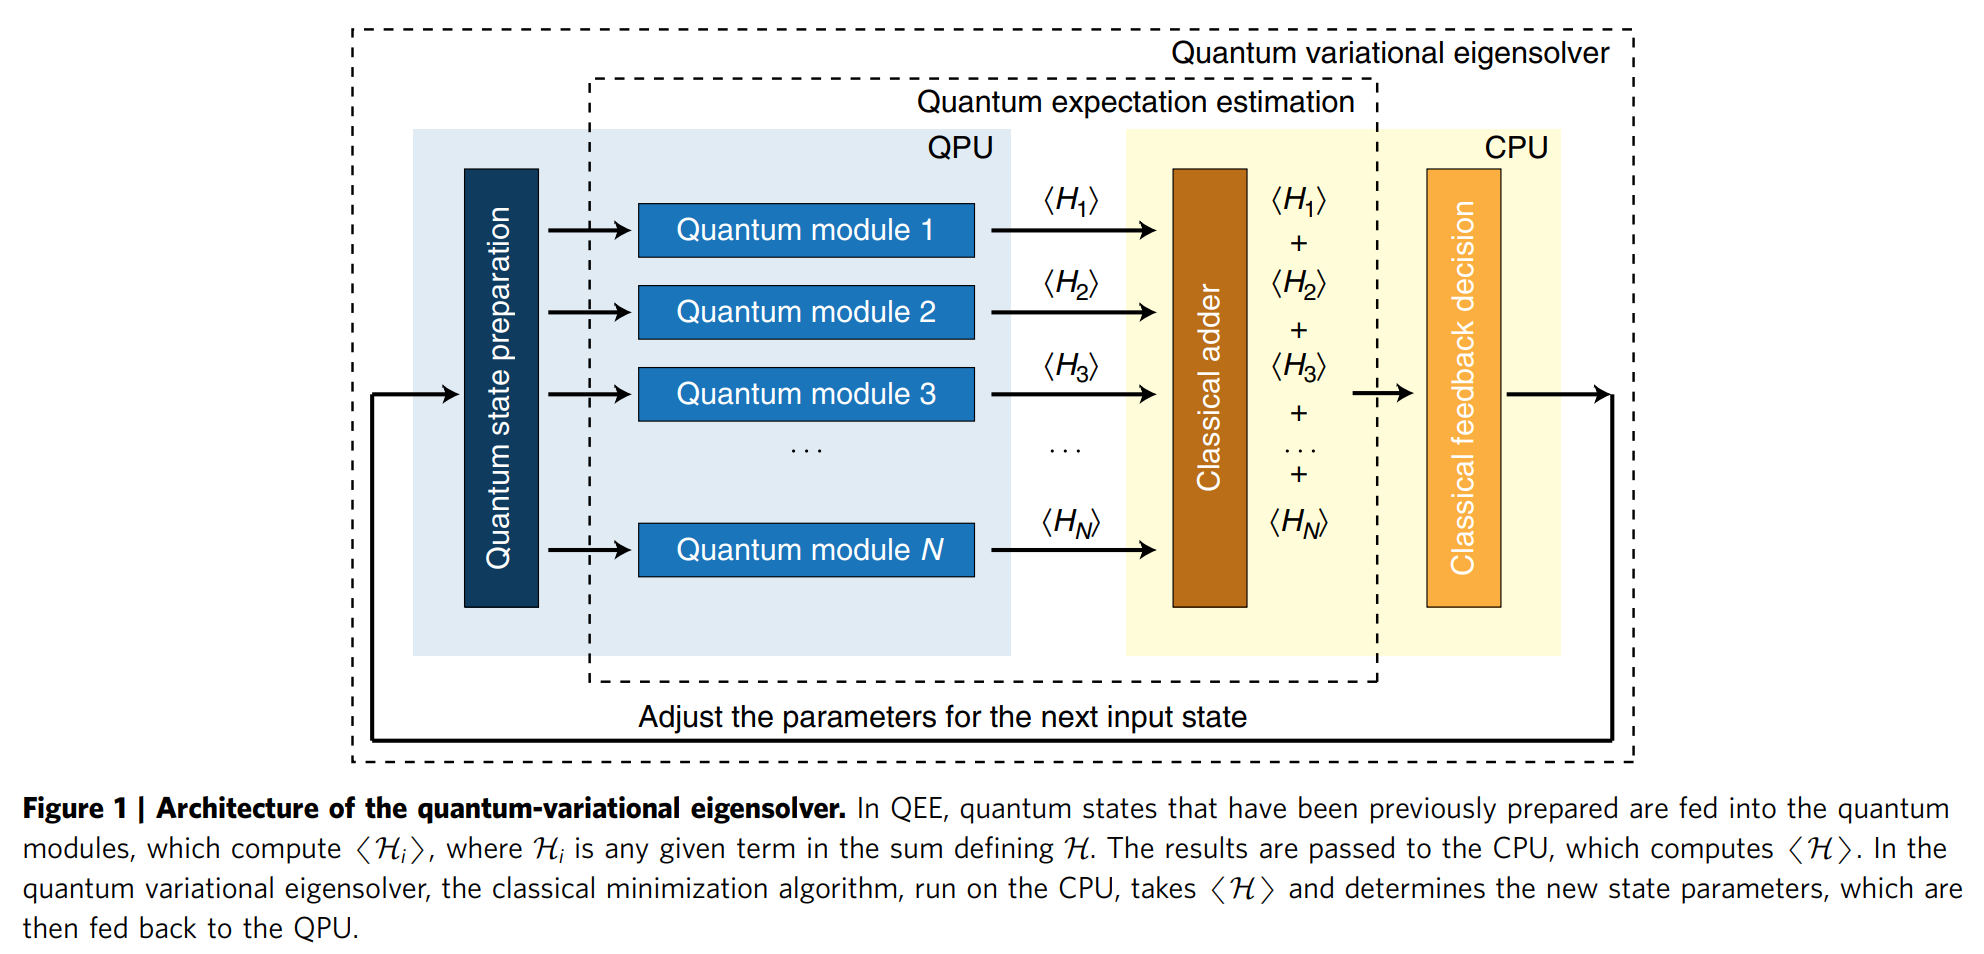
\includegraphics[scale=0.2]{qvei}
\end{figure}

It is well known that the eigenvalue problem for an observable
represented by an operator H can be restated as a variational
problem on the Rayleigh–Ritz quotient such that the eigenvector $\ket{\psi}$ corresponding to the lowest eigenvalue is the one hat minimizes
\begin{align}
\f{\bra{\psi} \had \ket{\psi}}{\braket{\psi}}
\end{align}
By varying the experimental parameters in the preparation of $\ket{\psi}$ and computing the Rayleigh–Ritz quotient using QEE as
a subroutine in a classical minimization, one may prepare
unknown eigenvectors. At the termination of the algorithm, a
simple prescription for the reconstruction of the eigenvector is
stored in the final set of experimental parameters that define $\ket{\psi}$. \\

Note that if a quantum state is characterized by an exponentially large
number of parameters, it cannot be prepared with a polynomial
number of operations. The set of efficiently preparable states are
therefore characterized by polynomially many parameters, and
we choose a particular set of ansatz states of this type.  Under
these conditions, a classical search algorithm on the experimental
parameters that define $\ket{\psi}$ needs only explore a polynomial
number of dimensions -- requirement for the search to be
efficient.\\

One example of a quantum state parameterized by a
polynomial number of parameters for which there is no known
efficient classical implementation is the unitary coupled cluster
ansatz
\begin{align}
\ket{\Psi} = e^{T - T^\dagger}\ket{\Phi}_\text{ref}
\end{align}
where $\ket{\Phi}_\text{ref}$ is some reference state, usually the Hartree Fock ground state, and $T$ is the cluster operator for an $N$ electron system, defined by
\begin{align}
T =T_1 + T_2 + \dots + T_N,
\end{align}
where
\begin{align}
T_1 = \sum_{pr}t^r_p \hat{a}_p^\dagger\hat{a}_r, \quad T_2 = \sum_{pqrs}t^{rs}_{pq}\hat{a}_p^\dagger \hat{a}_q^\dagger\hat{a}_r \hat{a}_s,\quad \dots
\end{align}
By construction, $(T - T^\dagger)$ is anti-Hermitian, and exponentiation maps it to a unitary operator $e^(T - T^\dagger)$. \\

For any fixed excitation level $k$, the reduced cluster operator is written as
\begin{align}
T^{(k)} = \sum^k_{i=1}T_i.
\end{align}
This state may be prepared efficiently on a quantum
device. The reduced anti-hermitian cluster operator  $(T^{(k)} - T^{(k)\dagger})$ is the sum of a polynomial number of terms—namely, it contains
a number of terms $\mathcal{O}(N^k(M-N)^k)$, where $M$ is the number of
single-particle orbitals. By defining an effective Hermitian
Hamiltonian $\had = i(T^{(k)} - T^{(k)\dagger})$ and performing the Jordan–
Wigner transformation to reach a Hamiltonian that acts on the
space of qubits $\hat{\had}$, we are left with a Hamiltonian that is a sum of polynomially many products of Pauli operators. The problem then reduces to the quantum simulation of this effective Hamiltonian, $\hat{\had}$ which can be one in polynomial time using known procedures. 





















\newpage




\section{Some Models in Quantum Statistical \& Condensed-Matter Physics}

\subsection{The Hubbard Model}

\subsection{The Ising Model}




\subsection{Transverse-field Ising model (quantum Ising model)}











\newpage




\section{Locality in Quantum Systems}

In this section we will look at this \href{https://arxiv.org/pdf/1008.5137.pdf}{\underline{paper}} by Matthew Hastings. This is actually a compilation of lecture notes focusing on the application of ideas of locality, in particular Lieb-Robinson bounds, to quantum many-body systems. For our purposes, we will only look at a few topics included. 
\begin{itemize}
	\item We want to understand ``locality'' in the context of quantum simulation. What, precisely, does it mean for a Hamiltonian to be ''local''? 
	
	\item What are the Lieb-Robinson bounds? 
	
	\item What is the Lieb-Schulz-Mattis theorem?
	
	\item What are topologically ordered states? 
\end{itemize}





\subsection{Introduction \& Notation}

The basic problem studied in quantum many-body theory is to find the properties of the ground state of a given
Hamiltonian. Expressed mathematically, the Hamiltonian $\had$ is a Hermitian matrix, and the ground state, which we write $\psi_0$, is an eigenvector of this matrix with the lowest eigenvalue.  The properties we are interested in studying
are expectation values of various observables: given a Hermitian matrix $O$, we would like to compute the expectation value $\langle \psi_0 , O \psi_0\rangle \equiv \langle O \rangle$. \\

While the method of ``exact diagonalization'' on a computer is an important technique in studying
quantum systems, it is only a small part of how physical problems are studied. The feature that distinguishes the study of quantum many-body systems is \textit{locality} of interactions. Consider a typical Hamiltonian, such as the one-dimensional transverse field Ising model TFIM):
\begin{align}
\had = -J \sum^{N-1}_{i=1}S^z_i S^z_{i+1} + B \sum^{N}_{i=1}S_i^x.
\end{align}
The very notation implicitly assumes local interactions. To be precise, throughout this section, we only consider quantum systems on a finite size lattice. We associate a $D$ dimensional Hilbert space with each lattice site, and the Hilbert space of the whole system is tensor product of these spaces. We use $N$ to represent the number of lattice sites, so that the Hilbert space on which a Hamiltonian such as the one above is defined in $D^N$ dimensions. A term such as $S^z_i S^z_{i+1}$ is short hand for $I_1 \otimes I_2 \otimes \dots \otimes S_i^z \otimes S^z_{i+1} \otimes I_{i+2} \otimes \dots \otimes I_N$, where $I_j$ is the identity operator on site $j$.\\

We let $i,j,k,\dots$ denote the lattice site, and $X,Y,Z$ to denote sets of lattice sites. We se $\Lambda$ to denote the set of all lattice sites. We use $\abs{X}$ to denote the cardinality of a set $X$. \\

An operator $O$ is supported on a set $A$ if we can write $O$ as a tensor product of two operators $O = I_{\Lambda\setminus A} \otimes P$, where $I_{\Lambda \setminus A}$ is the identity operator on the sites not in $A$ and $P$ is some operator defined on the $D^{\abs{A}}$ dimensional Hilbert space on the set $A$. For example, $S^z_i \otimes S^z_{i+1}$ is supported on the set $\{ i, i+1\}$. \\

We let $\norm{O}$ denote the ``operator norm'' for $O$. If $O$ is Hermitian, the operator norm is the equal to the absolute value of the largest eigenvalue of $O$. For arbitrary operators $O$, the operator norm is given by
\begin{align}
\norm{O} = \max_{\psi, \abs{\psi} = 1}  \abs{O \psi},
\end{align}
which one might have seen in real/functional analysis. \\

Using 2 simple assumptions: that the Hamiltonian has local interactions and that the Hamiltonian has a spectral gap, we will be able to prove a wide variety of results about the ground state of the Hamiltonian. We will consider two cases of a spectral gap: one where $E_1  - E_0 \geq \Delta E$, where $\Delta E$ is called the ``spectral gap.'' In the other case, we consider a Hamiltonian with several degenerate or approximately degenerate low energy states. \\

We will begin by considering properties of correlations in these systems, and prove an exponential decay of correlation functions. We then consider how the ground state of the system changes under a change in the Hamiltonian, and use this to prove a non-relativistic variant of Goldstone's Theorem. Finally, we apply these techniques to more interesting systems with topological order, beginning with the Lieb-Schultz-Mattis theorem However, before we can do any of this, we need to more precisely define the locality properties of the Hamiltonian and to prove a set of bounds on te propagation of information through the system called the Lieb-Robinson bounds. 



\subsection{Locality \& The Lieb-Robinson bounds}








\newpage


\section{Quantum Approximate Optimization Algorithm (QAOA)}

\newpage

\section{Quantum Variational Factorization (QVF)}

\newpage



\section{Variational Thermal Quantum Simulation via Thermofield Double States}



\subsection{Thermofield Double States (TFD)}


\newpage



\section{Generation of TFD and Critical Ground States with a Quantum Computer }



\newpage






\section{Efficient variational simulation of non-trivial quantum states}


In this section we look at this \href{https://arxiv.org/pdf/1803.00026.pdf}{\underline{paper}}, with title '' Efficient variational simulation of non-trivial quantum states.'' The idea is the following. The paper provides an efficient and general route for preparing \textit{non-trivial quantum states} (defined later) that are NOT adiabatically connected to unentangled product states. This approach will be a hybrid of quantum and classical variational protocols that incorporates a feedback loop between a quantum simulator and a classical computer. This turns out to be realizable on near-term quantum devices of synthetic quantum systems. \\

The paper provides explicit protocols which prepare with \textit{perfect fidelities} the following non-trivial quantum states: GHZ, quantum critical state, and topologically ordered state, with $L=2p$ variational parameters and physical runtimes $T \sim L$. \\

The paper also conjectures and numerically support (so, not analytically support) that the protocol can prepare with perfect fidelity and similar operational costs the ground state of every point in the 1D transverse field Ising model phase diagram (we will define this later). 




\subsection{Introduction}



The paper demonstrates the efficient preparation of certain non-trivial states using a variational hybrid quantum-classical simulation, which utilizes resources of a quantum simulator and a classical computer in a feedback loop. Given Hamiltonians realizable on a quantum simulator, a quantum state $\ket{\psi}(\bm{\gamma}, \bm{\beta})$ is produced with $(\bm{\gamma}, \bm\beta) \equiv (\gamma_1,\dots,\gamma_p, \beta_1,\dots,\beta_p)$ parameterizing a finite set of $2p$ variational angles (or times) that the Hamiltonians are run for. \\

A cost function, usually taken to be the energy of some target Hamiltonian, is then evaluated within the resulting state and optimized for in a classical computer, which yields a new set of $2p$ angles to be implemented to be fed back into the quantum simulator. \\

The entire process is iterated to convergence. \\


An example of an approach like this is the Quantum Approximate Optimization Algorithm (QAOA). There are a number of properties which make the variational quantum simulation appealing: it can be run on any quantum device (digital/tunable analog). The feedback loop of the protocol allows one to mitigate systematic errors that might be present in the experiment setups. \\

This variational quantum-classical simulations on local, uniform Hamiltonians can target GHZ state, the critical state of the 1D transverse field Ising model (TFIM), and the ground state of the 2d Toric code, all with \textit{perfect fidelity}. \\

Later, we will see that the entire ground state phase diagram of the TFIM can be produced with perfect fidelities and similar operational costs. This is only conjectured and numerically supported. \\

Finally, we will look at the preparation of the ground states of the antiferromagnetic (AFM) Heisenberg chains. We will see that the protocol is able to achieve them efficiently and with \textit{very good} fidelities (so, not perfect, but very good).



\subsection{Non-trivial quantum states}


In any case, let's look at some non-trivial quantum states. What are non-trivial quantum states? Consider a target state $\ket{\psi_t}$ and an untangled product state $\ket{\psi_u}$, both defined on a system with linear dimension $L$. $\ket{\psi_t}$ is said to be \textit{non-trivial} if there does not exist a \textit{local} unitary circuit $\U$ of finite depth that connects the two: $\ket{\psi_t} = \U \ket{\psi_u}$. Instead, the depth of a local unitary circuit connecting the two must be at least $\mathcal{O}(L^\al)$. \\

Intuitively, non-trivial states have entanglement patterns fundamentally different from product states, i.e., these are states that are very ``far'' from being product states. \\

From the perspective of local Hamiltonians and gaps, such states are separated from product states by a gap-closing phase transition in the thermodynamic limit, and thus preparing them with the quantum adiabatic algorithm is hard.\\


\begin{exmp}[GHZ states are non-trivial.] 
	Let's first look at what GHZ states are. GHZ stands for Greenberger-Horne-Zeilinger. GHZ is a certain type of entangled quantum state that involved at least three subsystems. Extremely non-classical properties of the state have been observed. \\
	
	\begin{defn}
		The GHZ state is an entangled quantum state of $M>2$ subsystems. If each system has dimension $d$, i.e., the local Hilbert space is isomorphic to $\mathbb{C}^d$, then th total Hilbert space of $M$ partite system is $\had_\text{tot} = (\mathbb{C}^d)^{\otimes M}$. This GHZ state is also named as $M$-partite qubit GHZ state, which reads
		\begin{align}
		\ket{\text{GHZ}} = \f{1}{\sqrt{d}}\sum^{d-1}_{i=0}\bigotimes \ket{i}.
		\end{align}
		In the case of each of the subsystems being two-dimensional, that is for qubits, it reads
		\begin{align}
		\ket{\text{GHZ}} = \f{\ket{0}^{\otimes M} + \ket{1}^{\otimes M}}{\sqrt{2}}.
		\end{align}
		The GHZ state is a quantum superposition of all qubits being in 0 with all being in 1. The GHZ state is a maximally entangled quantum state. The simplest being $\ket{\text{GHZ}} = (\ket{000} + \ket{111})/2$.\\
		
		GHZ states are in contrast to the so-called ``cat states,'' which are quantum superpositions of two macroscopically distinct states. Note that a cat state, unlike GHZ states, are not necessarily an entangled state because a cat state could be of one or more modes or particles. 
	\end{defn}
	
	
	
	
	Let us look at why the GHZ states are non-trivial. Consider the GHZ state:
	\begin{align}
	\ket{\text{GHZ}} = \f{1}{\sqrt{2}}\lp \bigotimes \ket{Z=1} + \bigotimes \ket{Z=-1} \rp.
	\end{align}
	Suppose there exists a local, finite-depth unitary $\U$ that takes the completely polarized product state $\ket{+} \equiv \bigotimes \ket{X=1}$ to $\ket{\text{GHZ}}$. Then due to locality, there exists a Lieb-Robinson bound which limits the spread of information and entanglement under this evolution, implying that $\U$ can  only generate a finite correlation length $\xi$ for the final state.  Measuring a long-range spin-spin correlator gives
	\begin{align}
	\bra{\text{GHZ}} Z_i Z_j \ket{\text{GHZ}} = 1,
	\end{align}
	while on the other hand the same quantity can be expressed as
	\begin{align}
	1 = \bra{+}\U^\dagger Z_i \U \U^\dagger Z_j \U \ket{+} ,
	\end{align}
	which in the limit $\abs{i-j} \gg \xi$ decomposes as
	\begin{align}
	\bra{+}\U^\dagger Z_i \U \ket{+} \bra{+} \U^\dagger Z_j \U \ket{+} = \bra{\text{GHZ}} Z_i \ket{\text{GHZ}} \bra{\text{GHZ}} Z_j \ket{\text{GHZ}} = 0\neq 1
	\end{align}
	which is a contradiction.
\end{exmp} 


Similar arguments apply to critical states which have polar-law correlations, and topologically ordered states which have long-range correlations in loop operators and non-zero topological entanglement entropy. 





 

\subsection{Variational Quantum-Classical Simulation (VQCS)}


Now, we define the variational quantum-classical simulation (VQCS). This is motivated by the QAOA and the VQE. \\


The protocol is envisioned to be run on a quantum simulator that can realize certain interactions between qubits and single qubit rotations, which we denote schematically by $H_1 , H_2$. The aim is to produce a good approximation to the ground state of a target many-body Hamiltonian $H_T$, which we will assume to be a linear combination of $H_1$ and $H_2$. \\

The VQCS begins with the ground state of $H_1$, denoted $\ket{\psi_1}$, and evolves it with the following sequence alternating between $H_1, H_2$:
\begin{align}
\ket{\psi(\bm\gamma, \bm\beta)}_p = e^{-i\beta_p H_1}e^{-i\gamma_p H_2}\dots e^{-i \beta_1 H_1}e^{-i \gamma_1 H_2}\ket{\psi_1}.
\end{align}

For a fixed integer $p$, there are $2p$ variational agles 
\begin{align}
(\bm\gamma, \bm\beta) \equiv (\gamma_1,\dots,\gamma_p, \beta_1,\dots, \beta_p).
\end{align}

A cost function, such as the energy expectation value of the target Hamiltonian
\begin{align}
F_p(\bm\gamma, \bm\beta) = _p\bra{ \psi(\bm\gamma,\bm\beta)} H_T \ket{\psi(\bm\gamma,\bm\beta)}_p,
\end{align}
is then evaluated. A classical computer then performs an optimization to produce a new set of angles (or times) $(\bm\gamma, \bm\beta)$ which are then fed back into the quantum simulator and the process is repeated until the cost function is desirably minimized. The state corresponding to these optimal angles is therefore the optimal state that can be prepared by the protocol given this cost function. \\


As the VQCS is envisioned to be run on near-term quantum simulators which are inherently noisy (NISQ), the physical runtimes $t = \sum^{p=L/2}_i (\gamma_i + \beta_i)$ of the VQCS constitute an important measure of the feasible of the protocol -- in general, shorter runtimes lead to less noise encountered and a better implementation.  













\subsection{Using VQCS to prepare nontrivial quantum states}

In this section we look at how the VQCS generates some non-trivial quantum states.


\subsubsection{GHZ state}

Recall the GHZ state looks like
\begin{align}
\ket{\text{GHZ}} = \f{1}{\sqrt{2}}\lp \bigotimes \ket{Z=1} + \bigotimes \ket{Z = -1} \rp.
\end{align} 
So it is a superposition of two possible ways that the system is completely aligned. The GHZ state can be taken to be the ground state of the following Hamiltonian
\begin{align}
\had_T = \sum^L_{i=1}Z_i Z_{i+1},
\end{align}
in the symmetry sector $S = \prod^L_{i}X_i =1$. Just to clarify the notation, $Z_i$ gives $+1$ when the state is ``up'', i.e., if the state is $\ket{\uparrow}$. This means the Hamiltonian ``favors'' (i.e., achieve lowest energy) when everybody is aligned. Further, for simplicity we assume periodic boundary conditions.\\

We choose in this case $H_1 = -\sum_i X_i$ with the product ground state $\ket{\psi_1} = \ket{+} = \bigotimes^L_{i}\ket{+}_i$. Recall that on the Bloch sphere, the $\ket{+}$ and $\ket{-}$ states lie in the horizontal plane, and are eigenstates of the $X$ operator, i.e., $X\ket{\pm} = \pm 1 \ket{\pm}$. We also know that $H_1$ has a straightforward implementation in both the analog and digital settings. \\

Next, choose $H_2 = \had_T$. On a digital quantum simulator, this can be achieved using elementary two-site gates $Z_i Z_{i+1}$: 
\begin{align}
e^{-i\gamma H_2} = \prod^{L/2}_{i=1} e^{-i\gamma Z_{2i}Z_{2i+1}}   \prod^{L/2}_{i=1} e^{-i\gamma Z_{2i-1}Z_{2i}}
\end{align}
such that...



 

\subsubsection{Critical State}

\subsubsection{Ground states of the TFIM at generic points in the phase diagram}

\subsubsection{Ground state of the Toric code}

\subsubsection{Ground state of AFM Heisenberg chain}











\subsection{Conclusions}


\subsection{Appendix}

\subsubsection{Optimal angles for preparing GHZ state at $p=L/2$}
\subsubsection{Explicit nonuniform unitary circuit for preparing the GHZ state}
\subsubsection{Energy optimization plot and optimal angles for preparing critical state at $p=L/2$}
\subsubsection{A Conjecture and Numerical Support}
\subsubsection{Numerical verification of preparation of Toric code ground state}
\subsubsection{Effect of errors on VQCS state preparation}






\newpage



\section{Measurement-based quantum computing: Briegel et al}

\href{https://www.nature.com/articles/nphys1157.pdf}{\underline{paper}}.


\newpage


\section{Mesurement-based quantum computing: Jozsa}




\href{https://arxiv.org/pdf/quant-ph/0508124.pdf}{\underline{paper}}





\end{document}
